\documentclass[../../main-ap-physics.tex]{subfiles}

\begin{document}

\section{Two-Dimensional Kinematics}

\subsection{Kinematics in Two Dimensions: An Introduction}

\subsubsection*{Two-Dimensional Motion: Walking in a City}

Suppose you want to walk from one point to another in a city with uniform square blocks, as pictured in Figure \ref{5wAnWT}

\begin{center}
    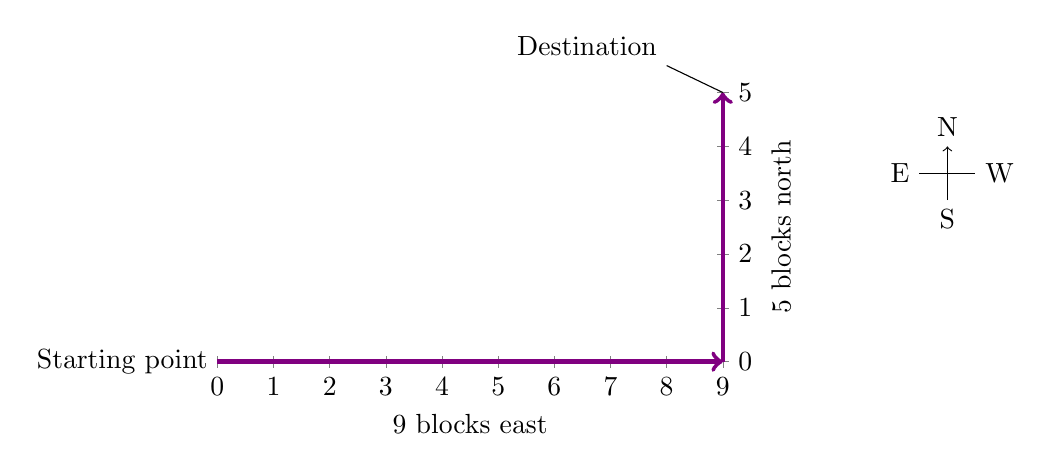
\begin{tikzpicture}
        \begin{axis}[width=8cm, height=5cm,
            xmin=0,xmax=9,
            ymin=0,ymax=5,
            xtick={0,1,...,9},
            ytick={0,1,...,5},
            clip=false,
            axis y line = right,
            axis x line = left,
            xlabel={9 blocks east},
            ylabel={5 blocks north},
        ]
        \draw[->,ultra thick,violet] (0,0) -- (9,0);
        \draw[->,ultra thick,violet] (9,0) -- ++(0,5);
        \node[left] at (0,0) {Starting point};
        \draw (9,5) -- ++(-1,0.5) node[above left] {Destination};
        \begin{scope}[shift={(13,3)}]
            \draw[->] (0,0) node[below] {S} -- ++(0,1) node[above] {N};
            \draw (-0.5,0.5) node[left] {E} -- ++(1,0) node [right] {W};
        \end{scope}
        \end{axis}
    \end{tikzpicture}
    \captionsetup{type=figure,margin=1in,font=scriptsize}
    \captionof{figure}{A pedestrian walks a two-dimensional path between two points in a city. In this scene, all blocks are square and are the same size.}
    \label{5wAnWT}
\end{center}

The straight-line path that a helicopter might fly is blocked to you as a pedestrian, and so you are forced to take a two-dimensional path, such as the one shown. You walk 14 blocks in all, 9 east followed by 5 north. What is the straight-line distance?

\vspace{1em}

An old adage states that the shortest distance between two points is a straight line. The two legs of the trip and the straight-line path form a right triangle, and so the Pythagorean theorem,  $a^2 + b^2 = c^2$, can be used to find the straight-line distance.

\begin{equation}
    a^2 + b^2 = c^2
\end{equation}

\begin{center}
    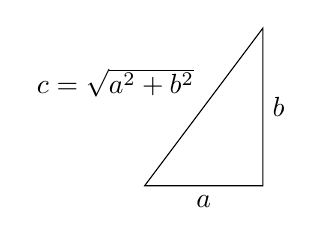
\begin{tikzpicture}
        \draw (0,0) -- (1.5,0) node[pos=0.5,below] {$a$} -- ++(0,2) node[pos=0.5,right] {$b$} -- cycle node[pos=0.5,above left] {$c = \sqrt{a^2 + b^2}$};
    \end{tikzpicture}
    \captionsetup{type=figure,margin=1in,font=scriptsize}
    \captionof{figure}{The Pythagorean theorem relates the length of the legs of a right triangle, labeled $a$ and $b$, with the hypotenuse, labeled $c$. The relationship is given by: $a^2 + b^2 = c^2$. This can be rewritten, solving for $c$: $c = \sqrt{a^2 + b^2}$.}
\end{center}

The hypotenuse of the triangle is the straight-line path, and so in this case its length in units of city blocks is 

\begin{equation*}
    \sqrt{\left(\SI{9}{blocks}\right)^2 + \left(\SI{5}{blocks}\right)^2} = \SI{10.3}{blocks}
\end{equation*}

considerably shorter than the 14 blocks you walked. (Note that we are using three significant figures in the answer. Although it appears that ``9'' and ``5'' have only one significant digit, they are discrete numbers. In this case ``9 blocks'' is the same as ``9.0 or 9.00 blocks.'' We have decided to use three significant figures in the answer in order to show the result more precisely.)

\begin{center}
    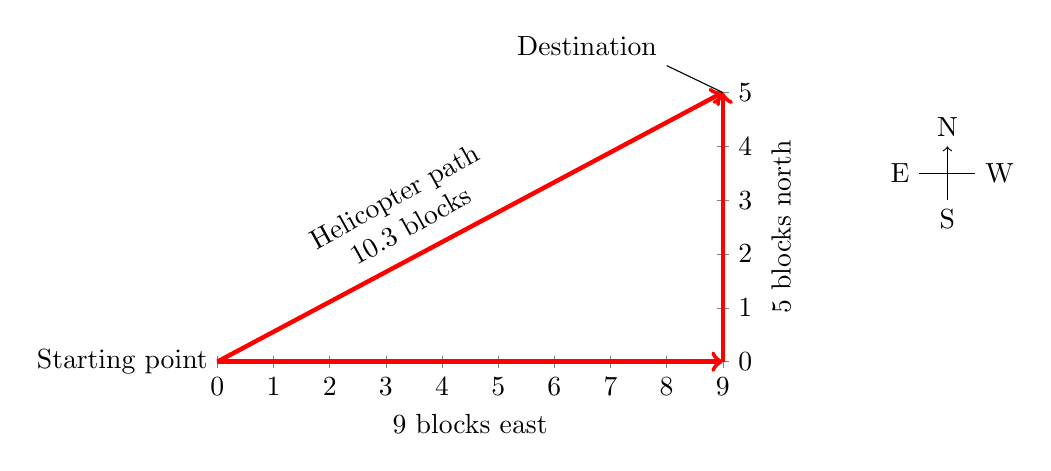
\begin{tikzpicture}
        \begin{axis}[width=8cm, height=5cm,
            xmin=0,xmax=9,
            ymin=0,ymax=5,
            xtick={0,1,...,9},
            ytick={0,1,...,5},
            clip=false,
            axis y line = right,
            axis x line = left,
            xlabel={9 blocks east},
            ylabel={5 blocks north},
        ]
        \draw[->,ultra thick,red] (0,0) -- (9,0);
        \draw[->,ultra thick,red] (9,0) -- ++(0,5);
        \draw[->,ultra thick,red] (0,0) -- (9,5) node[pos=0.6, above left=1mm,rotate=29,align=center,black] {Helicopter path\\10.3 blocks} node[black,below,pos=0.5,rotate=29] {\Large \myheli};
        \node[left] at (0,0) {Starting point};
        \draw (9,5) -- ++(-1,0.5) node[above left] {Destination};
        \begin{scope}[shift={(13,3)}]
            \draw[->] (0,0) node[below] {S} -- ++(0,1) node[above] {N};
            \draw (-0.5,0.5) node[left] {E} -- ++(1,0) node [right] {W};
        \end{scope}
        \end{axis}
    \end{tikzpicture}
    \captionsetup{type=figure,margin=1in,font=scriptsize}
    \captionof{figure}{The straight-line path followed by a helicopter between the two points is shorter than the 14 blocks walked by the pedestrian. All blocks are square and the same size.}
    \label{R2c4pp}
\end{center}

The fact that the straight-line distance (10.3 blocks) in Figure \ref{R2c4pp} is less than the total distance walked (14 blocks) is one example of a general characteristic of vectors. (Recall that \gls{vector}s are quantities that have both magnitude and direction.)

\vspace{1em}

As for one-dimensional kinematics, we use arrows to represent vectors. The length of the arrow is proportional to the vector's magnitude. The arrow's length is indicated by hash marks in Figure \ref{5wAnWT} and Figure \ref{R2c4pp}. The arrow points in the same direction as the vector. For two-dimensional motion, the path of an object can be represented with three vectors: one vector shows the straight-line path between the initial and final points of the motion, one vector shows the horizontal component of the motion, and one vector shows the vertical component of the motion. The horizontal and vertical components of the motion add together to give the straight-line path. For example, observe the three vectors in Figure \ref{R2c4pp}. The first represents a 9-block displacement east. The second represents a 5-block displacement north. These vectors are added to give the third vector, with a 10.3-block total displacement. The third vector is the straight-line path between the two points. Note that in this example, the vectors that we are adding are perpendicular to each other and thus form a right triangle. This means that we can use the Pythagorean theorem to calculate the magnitude of the total displacement. (Note that we cannot use the Pythagorean theorem to add vectors that are not perpendicular. We will develop techniques for adding vectors having any direction, not just those perpendicular to one another, in ``Vector Addition and Subtraction: Graphical Methods and Vector Addition and Subtraction: Analytical Methods.'')

\subsubsection*{The Independence of Perpendicular Motions}

The person taking the path shown in Figure \ref{R2c4pp} walks east and then north (two perpendicular directions). How far they walk east is only affected by their motion eastward. Similarly, how far they walk north is only affected by their motion northward.

\begin{gradient}{INDEPENDENCE OF MOTION}
    The horizontal and vertical components of two-dimensional motion are independent of each other. Any motion in the horizontal direction does not affect motion in the vertical direction, and vice versa.
\end{gradient}

This is true in a simple scenario like that of walking in one direction first, followed by another. It is also true of more complicated motion involving movement in two directions at once. For example, let's compare the motions of two baseballs. One baseball is dropped from rest. At the same instant, another is thrown horizontally from the same height and follows a curved path. A stroboscope has captured the positions of the balls at fixed time intervals as they fall.

\begin{center}
    \begin{tikzpicture}
        \begin{axis}[width=7cm,height=8cm,ticks=none,
        axis lines = center,
        axis line style={draw=none},
        clip=false,
        xmin=0, xmax=120,
        ymin=0, ymax=70,
        ]
        % \draw[only marks,domain=0:100,variable=\x,samples=200] plot ({\x},{patheq(\x,60,28.6,0)});
        % \draw[dashed] (0,{patheq(0,60,28.6,0)}) -- ++(100,0);
        % \draw[dashed] (0,{patheq(0,60,28.6,0)}) -- ++(0,-{patheq(0,60,28.6,0)});
        
        \pgfplotsinvokeforeach{20,40,60,80,100}{
            \draw[thick,Green,->] (#1,{patheq(#1,60,28.6,0)}) -- ++(0,-0.2*#1);
            \draw[thick,->] (#1,{patheq(#1,60,28.6,0)}) -- ++(15,0);
            \fill[RoyalBlue] (#1,{patheq(#1,60,28.6,0)}) circle (3pt);
            
            \draw[dashed] (0,{patheq(#1,60,28.6,0)}) -- ++(#1,0);

            \draw[thick,Green,->] (0,{patheq(#1,60,28.6,0)}) -- ++(0,-0.2*#1);
            \fill[red] (0,{patheq(#1,60,28.6,0)}) circle (3pt);
        }
        \end{axis}
    \end{tikzpicture}
    \captionsetup{type=figure,margin=1in,font=scriptsize}
    \captionof{figure}{This shows the motions of two identical balls—one falls from rest, the other has an initial horizontal velocity. Each subsequent position is an equal time interval. Arrows represent horizontal and vertical velocities at each position. The ball on the right has an initial horizontal velocity, while the ball on the left has no horizontal velocity. Despite the difference in horizontal velocities, the vertical velocities and positions are identical for both balls. This shows that the vertical and horizontal motions are independent.}
    \label{iZGL98}
\end{center}

It is remarkable that for each flash of the strobe, the vertical positions of the two balls are the same. This similarity implies that the vertical motion is independent of whether or not the ball is moving horizontally. (Assuming no air resistance, the vertical motion of a falling object is influenced by gravity only, and not by any horizontal forces.) Careful examination of the ball thrown horizontally shows that it travels the same horizontal distance between flashes. This is due to the fact that there are no additional forces on the ball in the horizontal direction after it is thrown. This result means that the horizontal velocity is constant, and affected neither by vertical motion nor by gravity (which is vertical). Note that this case is true only for ideal conditions. In the real world, air resistance will affect the speed of the balls in both directions.

\vspace{1em}

The two-dimensional curved path of the horizontally thrown ball is composed of two independent one-dimensional motions (horizontal and vertical). The key to analyzing such motion, called projectile motion, is to resolve (break) it into motions along perpendicular directions. Resolving two-dimensional motion into perpendicular components is possible because the components are independent. We shall see how to resolve vectors in ``Vector Addition and Subtraction: Graphical Methods'' and ``Vector Addition and Subtraction: Analytical Methods.'' We will find such techniques to be useful in many areas of physics.

\begin{gradient}{PHET EXPLORATIONS}
    \textbf{Ladybug Motion 2D}: Learn about position, velocity and acceleration vectors. Move the ladybug by setting the position, velocity or acceleration, and see how the vectors change. Choose linear, circular or elliptical motion, and record and playback the motion to analyze the behavior.

    \vspace{1em}

    \href{https://openstax.org/l/28ladybugmotion}{Click to view content}.
\end{gradient}

\subsection{Vector Addition and Subtraction: Graphical Methods}

\subsubsection*{Vectors in Two Dimensions}

A \gls{vector} is a quantity that has magnitude and direction. Displacement, velocity, acceleration, and force, for example, are all vectors. In one-dimensional, or straight-line, motion, the direction of a vector can be given simply by a plus or minus sign. In two dimensions (2-d), however, we specify the direction of a vector relative to some reference frame (i.e., coordinate system), using an arrow having length proportional to the vector's magnitude and pointing in the direction of the vector.

\vspace{1em}
Figure \ref{huatRZ} shows such a graphical representation of a vector, using as an example the total displacement for the person walking in a city considered in Kinematics in Two Dimensions: An Introduction. We shall use the notation that a boldface symbol, such as $\mathbf{D}$, stands for a vector. Its magnitude is represented by the symbol in italics, \textbf{\textit{D}}, and its direction by $\theta$.

\begin{gradient}{VECTORS IN THIS TEXT}
    In this text, we will represent a vector with a boldface variable. For example, we will represent the quantity force with the vector $\textbf{F}$, which has both magnitude and direction. The magnitude of the vector will be represented by a variable in italics, such as \textbf{\textit{F}}, and the direction of the variable will be given by an angle $\theta$.
\end{gradient}

\begin{center}
    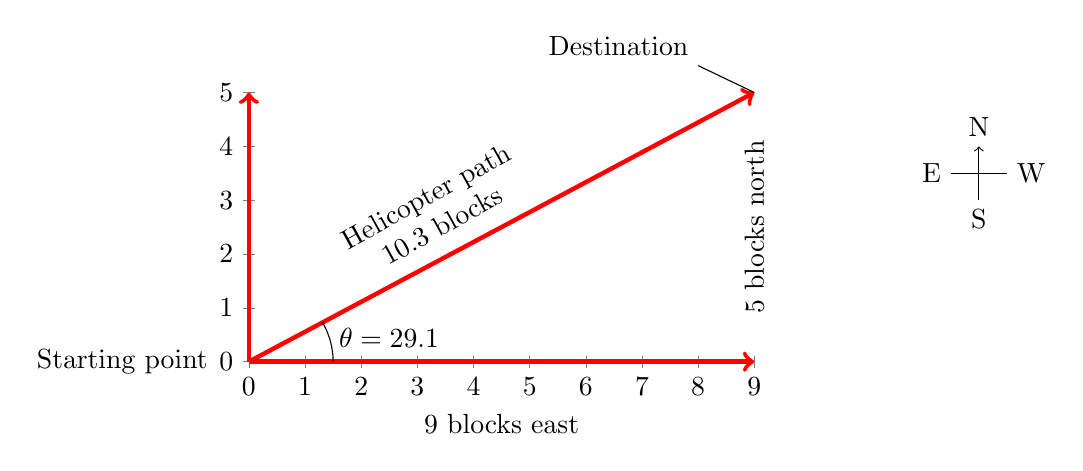
\begin{tikzpicture}
        \begin{axis}[width=8cm, height=5cm,
            xmin=0,xmax=9,
            ymin=0,ymax=5,
            xtick={0,1,...,9},
            ytick={0,1,...,5},
            clip=false,
            axis lines = left,
            xlabel={9 blocks east},
        ]
        \draw[->,ultra thick,red] (0,0) -- (9,0);
        \draw[->,ultra thick,red] (0,0) -- ++(0,5);
        \draw[->,ultra thick,red] (0,0) -- (9,5) node[pos=0.6, above left=1mm,rotate=29,align=center,black] {Helicopter path\\10.3 blocks} node[black,below,pos=0.5,rotate=29] {\Large \myheli};
        \node[left=4mm] at (0,0) {Starting point};
        \draw (9,5) -- ++(-1,0.5) node[above left] {Destination};
        \draw (1.5,0) arc (0:29.1:1.5) node[right,pos=0.6] {$\theta = \ang{29.1}$};
        \node[rotate=90] at (9,2.5) {5 blocks north};
        \begin{scope}[shift={(13,3)}]
            \draw[->] (0,0) node[below] {S} -- ++(0,1) node[above] {N};
            \draw (-0.5,0.5) node[left] {E} -- ++(1,0) node [right] {W};
        \end{scope}
        \end{axis}
    \end{tikzpicture}
    \captionsetup{type=figure,margin=1in,font=scriptsize}
    \captionof{figure}{A person walks 9 blocks east and 5 blocks north. The displacement is 10.3 blocks at an angle \ang{29.1} north of east.} 
    \label{huatRZ}
\end{center}

\begin{center}
    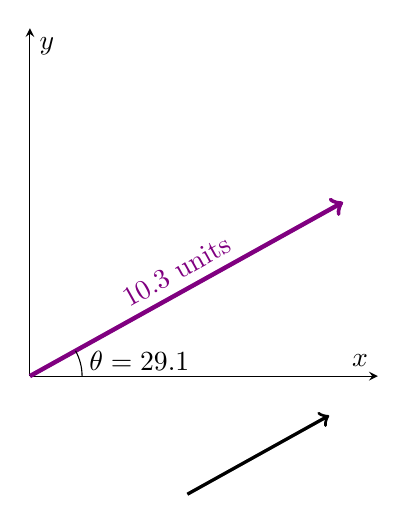
\begin{tikzpicture}
        \begin{axis}[width=6cm,height=6cm,
            xmin=0,xmax=10,
            ymin=0,ymax=10,
            ticks=none,
            axis lines=center,
            xlabel={$x$},
            ylabel={$y$},
            clip=false
        ]
        \draw[ultra thick,violet,->] (0,0) -- ++(9,5) node[pos=0.5,above,rotate=29.1] {10.3 units};
        \draw (1.5,0) arc (0:29:1.5) node[pos=0.6,right] {$\theta = \ang{29.1}$};
        \end{axis}
        \tkzRegle[Fond=true,Opacite=0.9,CouleurFond=yellow,AfficheValeurs=false,Origine={(-0.5,1)},Echelle=0.4,Rotation=29.1]
        \tkzRapporteur[Fond,CouleurFond=blue,Echelle=0.3,Origine={(2,-1.5)},AfficheAngles=false]
        \draw[very thick,->] (2,-1.5) -- ++(0.2*9,0.2*5);
    \end{tikzpicture}
    \captionsetup{type=figure,margin=1in,font=scriptsize}
    \captionof{figure}{To describe the resultant vector for the person walking in a city considered in Figure \ref{huatRZ} graphically, draw an arrow to represent the total displacement vector $\textbf{D}$. Using a protractor, draw a line at an angle $\theta$ relative to the east-west axis. The length \textbf{\textit{D}} of the arrow is proportional to the vector's magnitude and is measured along the line with a ruler. In this example, the magnitude \textbf{\textit{D}} of the vector is 10.3 units, and the direction $\theta$ is \ang{29.1} north of east.}
\end{center}

\subsubsection*{Vector Addition: Head-to-Tail Method}

The \gls{head-to-tail method} is a graphical way to add vectors, described in Figure \ref{SNgwC3} below and in the steps following. The \gls{tail} of the vector is the starting point of the vector, and the \gls{head} (or tip) of a vector is the final, pointed end of the arrow.

\begin{center}
    \begin{tikzpicture}
        \begin{axis}[width=6cm,height=6cm,
            xmin=0,xmax=11,
            ymin=0,ymax=11,
            axis lines=center,
            xlabel={$x$},
            ylabel={$y$},
            clip=false,
            xtick={0,1,...,9},
            ytick=\empty,
            xticklabels={},
        ]
        \draw[ultra thick,violet,->] (0,0) -- ++(9,0) node[pos=0.2,above,black] {$\theta = \ang{0}$} node[pos=0.7,above=2pt,black] {9 units};
        \end{axis}
    \end{tikzpicture}%
    \hspace{2em}
    \begin{tikzpicture}
        \begin{axis}[width=6cm,height=6cm,
            xmin=0,xmax=11,
            ymin=0,ymax=11,
            axis lines=center,
            xlabel={$x$},
            ylabel={$y$},
            clip=false,
            xtick={9},
            ytick=\empty,
            xticklabels={},
        ]
        \draw[ultra thick,violet,->] (0,0) -- ++(9,0);
        \draw[ultra thick,violet,->] (9,0) -- ++(0,5);
        \end{axis}
    \end{tikzpicture}%
    \hspace{2em}
    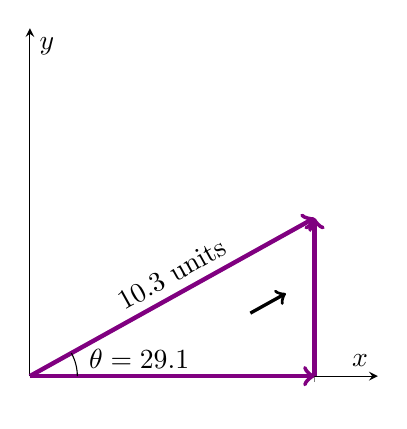
\begin{tikzpicture}
        \begin{axis}[width=6cm,height=6cm,
            xmin=0,xmax=11,
            ymin=0,ymax=11,
            axis lines=center,
            xlabel={$x$},
            ylabel={$y$},
            clip=false,
            xtick={9},
            ytick=\empty,
            xticklabels={},
        ]
        \draw[ultra thick,violet,->] (0,0) -- ++(9,0);
        \draw[ultra thick,violet,->] (9,0) -- ++(0,5);
        \draw[ultra thick,violet,->] (0,0) -- (9,5) node[pos=0.75,above left,rotate=29.1,black] {10.3 units};
        \draw (1.5,0) arc (0:29.1:1.5) node[pos=0.75,right=2pt] {$\theta = \ang{29.1}$};
        \end{axis}
    \tkzRegle[Fond=true,Opacite=0.9,CouleurFond=yellow,AfficheValeurs=false,Origine={(0.2,1.2)},Echelle=0.3,Rotation=29.1]
        \tkzRapporteur[Fond,CouleurFond=blue,Echelle=0.1,Origine={(2.8,0.8)},AfficheAngles=false]
        \draw[very thick,->] (2.8,0.8) -- ++(0.05*9,0.05*5);
    \end{tikzpicture}
    \captionsetup{type=figure,margin=1in,font=scriptsize}
    \captionof{figure}{\textbf{Head-to-Tail Method}: The head-to-tail method of graphically adding vectors is illustrated for the two displacements of the person walking in a city considered in Figure \ref{huatRZ}. (a) Draw a vector representing the displacement to the east. (b) Draw a vector representing the displacement to the north. The tail of this vector should originate from the head of the first, east-pointing vector. (c) Draw a line from the tail of the east-pointing vector to the head of the north-pointing vector to form the sum or \gls{resultant vector} $\textbf{D}$. The length of the arrow $\textbf{D}$ is proportional to the vector’s magnitude and is measured to be 10.3 units . Its direction, described as the angle with respect to the east (or horizontal axis) $\theta$ is measured with a protractor to be \ang{29.1}.}
    \label{SNgwC3}
\end{center}

\textbf{Step 1}. \textit{Draw an arrow to represent the first vector (9 blocks to the east) using a ruler and protractor.}

\begin{center}
    \begin{tikzpicture}
        \begin{axis}[width=6cm,height=6cm,
            xmin=0,xmax=11,
            ymin=0,ymax=11,
            axis lines=center,
            xlabel={$x$},
            ylabel={$y$},
            clip=false,
            xtick={0,1,...,9},
            ytick=\empty,
            xticklabels={},
        ]
        \draw[ultra thick,violet,->] (0,0) -- ++(9,0) node[pos=0.2,above,black] {$\theta = \ang{0}$} node[pos=0.7,above=2pt,black] {9 units};
        \end{axis}
    \end{tikzpicture}
\end{center}

\textbf{Step 2}. Now draw an arrow to represent the second vector (5 blocks to the north). \textit{Place the tail of the second vector at the head of the first vector}.

\begin{center}
    \begin{tikzpicture}
        \begin{axis}[width=6cm,height=6cm,
            xmin=0,xmax=11,
            ymin=0,ymax=11,
            axis lines=center,
            xlabel={$x$},
            ylabel={$y$},
            clip=false,
            xtick={9},
            ytick=\empty,
            xticklabels={},
        ]
        \draw[ultra thick,violet,->] (0,0) -- ++(9,0);
        \draw[ultra thick,violet,->] (9,0) -- ++(0,5);
        \end{axis}
    \end{tikzpicture}
\end{center}

\textbf{Step 3}. \textit{If there are more than two vectors, continue this process for each vector to be added. Note that in our example, we have only two vectors, so we have finished placing arrows tip to tail.}

\vspace{1em}

\textbf{Step 4}. \textit{Draw an arrow from the tail of the first vector to the head of the last vector}. This is the resultant, or the sum, of the other vectors.

\begin{center}
    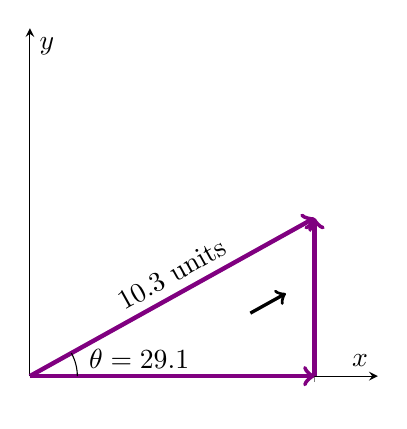
\begin{tikzpicture}
        \begin{axis}[width=6cm,height=6cm,
            xmin=0,xmax=11,
            ymin=0,ymax=11,
            axis lines=center,
            xlabel={$x$},
            ylabel={$y$},
            clip=false,
            xtick={9},
            ytick=\empty,
            xticklabels={},
        ]
        \draw[ultra thick,violet,->] (0,0) -- ++(9,0);
        \draw[ultra thick,violet,->] (9,0) -- ++(0,5);
        \draw[ultra thick,violet,->] (0,0) -- (9,5) node[pos=0.75,above left,rotate=29.1,black] {10.3 units};
        \draw (1.5,0) arc (0:29.1:1.5) node[pos=0.75,right=2pt] {$\theta = \ang{29.1}$};
        \end{axis}
    \tkzRegle[Fond=true,Opacite=0.9,CouleurFond=yellow,AfficheValeurs=false,Origine={(0.2,1.2)},Echelle=0.3,Rotation=29.1]
        \tkzRapporteur[Fond,CouleurFond=blue,Echelle=0.1,Origine={(2.8,0.8)},AfficheAngles=false]
        \draw[very thick,->] (2.8,0.8) -- ++(0.05*9,0.05*5);
    \end{tikzpicture}
\end{center}

\textbf{Step 5}. \textit{To get the magnitude of the resultant, measure its length with a ruler. (Note that in most calculations, we will use the Pythagorean theorem to determine this length.)}

\vspace{1em}

\textbf{Step 6}. \textit{To get the direction of the resultant, measure the angle it makes with the reference frame using a protractor. (Note that in most calculations, we will use trigonometric relationships to determine this angle.)}

\vspace{1em}

The graphical addition of vectors is limited in accuracy only by the precision with which the drawings can be made and the precision of the measuring tools. It is valid for any number of vectors.

\begin{example}
    \textit{Adding Vectors Graphically Using the Head-to-Tail Method: A Woman Takes a Walk}. Use the graphical technique for adding vectors to find the total displacement of a person who walks the following three paths (displacements) on a flat field. First, she walks \SI{25.0}{m} in a direction  \ang{49.0} north of east. Then, she walks \SI{23.0}{m} heading \ang{15.0} north of east. Finally, she turns and walks \ang{32.0}{m} in a direction \ang{68.0} south of east.
\end{example}

\Solution \textit{Strategy}: Represent each displacement vector graphically with an arrow, labeling the first $\textbf{A}$, the second $\textbf{B}$, and the third  $\textbf{C}$, making the lengths proportional to the distance and the directions as specified relative to an east-west line. The head-to-tail method outlined above will give a way to determine the magnitude and direction of the resultant displacement, denoted $\textbf{R}$.

\vspace{1em}

(1) Draw the three displacement vectors.

\begin{center}
    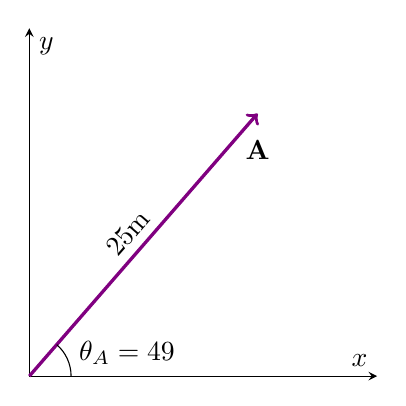
\begin{tikzpicture}
        \begin{axis}[width=6cm,height=6cm,
            xmin=0,xmax=25,
            ymin=0,ymax=25,
            clip=false,
            ylabel=$y$,
            xlabel=$x$,
            ticks=none,
            axis lines=center
        ]
        \draw[very thick,->,violet] (0,0) -- ({25*cos(49)},{25*sin(49)}) node[pos=0.6,black,above left,rotate=49] {\SI{25}{m}} node[black,below=2mm] {$\textbf{A}$};
        \draw (3,0) arc (0:49:3) node[pos=0.7,right=2pt] {$\theta_{\text{A}} = \ang{49}$};
        \end{axis}
    \end{tikzpicture}%
    \hspace{2em}
    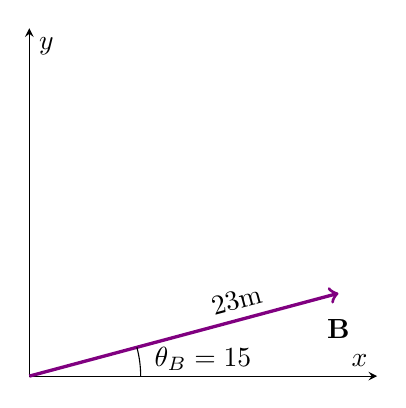
\begin{tikzpicture}
        \begin{axis}[width=6cm,height=6cm,
            xmin=0,xmax=25,
            ymin=0,ymax=25,
            clip=false,
            ylabel=$y$,
            xlabel=$x$,
            ticks=none,
            axis lines=center
        ]
        \draw[very thick,->,violet] (0,0) -- ({23*cos(15)},{23*sin(15)}) node[pos=0.8,black,above left,rotate=15] {\SI{23}{m}} node[black,below=2mm] {$\textbf{B}$};
        \draw (8,0) arc (0:15:8) node[pos=0.6,right=2pt] {$\theta_{\text{B}} = \ang{15}$};
        \end{axis}
    \end{tikzpicture}%
    \hspace{2em}
    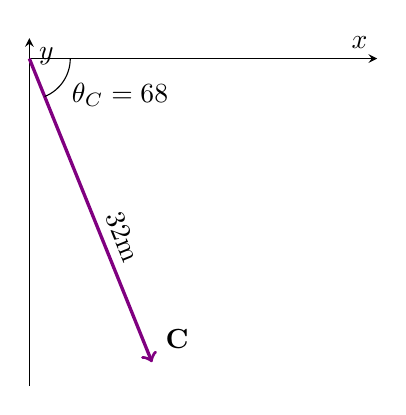
\begin{tikzpicture}
        \begin{axis}[width=6cm,height=6cm,
            xmin=0,xmax=34,
            ymin=-32,ymax=2,
            clip=false,
            ylabel=$y$,
            xlabel=$x$,
            ticks=none,
            axis lines=center,
            clip=false,
        ]
        \draw[very thick,->,violet] (0,0) -- ({32*cos(-68)},{32*sin(-68)}) node[pos=0.5,black,above right,rotate=-68] {\SI{32}{m}} node[black,above right=1pt] {$\textbf{C}$};
        \draw (4,0) arc (0:-68:4) node[pos=0.08,right=-1mm] {$\theta_{\text{C}} = \ang{68}$};
        \end{axis}
    \end{tikzpicture}
\end{center}

(2) Place the vectors head to tail retaining both their initial magnitude and direction.

\begin{center}
    \begin{tikzpicture}
    
        \begin{axis}[width=12cm,height=6cm,
            xmin=0,xmax=60,
            ymin=0,ymax=30,
            axis lines=center,
            ticks=none,
            clip=false,
            ylabel=$y$,
            xlabel=$x$,
            clip=false,
        ]
        \coordinate (A) at ({25*cos(49)},{25*sin(49)});
        \coordinate (B) at ({23*cos(15)},{23*sin(15)});
        \coordinate (AB) at ({25*cos(49)+23*cos(15)},{25*sin(49)+23*sin(15)});
        \coordinate (C) at ({32*cos(-68)},{32*sin(-68)});
        \coordinate (R) at ({50.8*cos(-5.47)},{50.8*sin(-5.47)});
        
        \draw[very thick,violet,->] (0,0) -- (A) node[black,pos=0.5,below=1mm] {$\textbf{A}$};
        \draw[very thick,violet,->] (A) -- ++(B) node[pos=0.5,black,below=1mm] {$\textbf{B}$};
        \draw[very thick,violet,->] (AB) -- ++(C) node[pos=0.5,black,right=1mm] {$\textbf{C}$};
        \end{axis}
    \end{tikzpicture}
\end{center}

(3) Draw the resultant vector,  $\textbf{R}$.

\begin{center}
    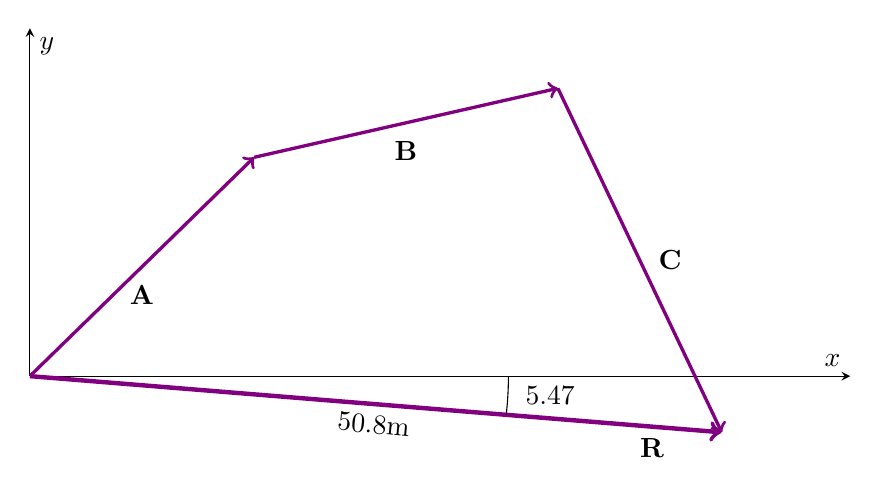
\begin{tikzpicture}
        \begin{axis}[width=12cm,height=6cm,
            xmin=0,xmax=60,
            ymin=0,ymax=30,
            axis lines=center,
            ticks=none,
            clip=false,
            ylabel=$y$,
            xlabel=$x$,
            clip=false,
        ]
        \coordinate (A) at ({25*cos(49)},{25*sin(49)});
        \coordinate (B) at ({23*cos(15)},{23*sin(15)});
        \coordinate (AB) at ({25*cos(49)+23*cos(15)},{25*sin(49)+23*sin(15)});
        \coordinate (C) at ({32*cos(-68)},{32*sin(-68)});
        \coordinate (R) at ({50.8*cos(-5.47)},{50.8*sin(-5.47)});
        
        \draw[very thick,violet,->] (0,0) -- (A) node[black,pos=0.5,below=1mm] {$\textbf{A}$};
        \draw[very thick,violet,->] (A) -- ++(B) node[pos=0.5,black,below=1mm] {$\textbf{B}$};
        \draw[very thick,violet,->] (AB) -- ++(C) node[pos=0.5,black,right=1mm] {$\textbf{C}$};
        \draw[ultra thick,violet,->] (0,0) -- (R) node[black,pos=0.5,below,rotate=-5.47] {\SI{50.8}{m}} node[pos=0.9,below,black] {$\textbf{R}$};
        \draw (35,0) arc (0:-5.47:35) node[pos=0.5,right=1mm] {\ang{5.47}};
        \end{axis}
    \end{tikzpicture}
\end{center}

(4) Use a ruler to measure the magnitude of $\textbf{R}$, and a protractor to measure the direction of $\textbf{R}$. While the direction of the vector can be specified in many ways, the easiest way is to measure the angle between the vector and the nearest horizontal or vertical axis. Since the resultant vector is south of the eastward pointing axis, we flip the protractor upside down and measure the angle between the eastward axis and the vector.

\begin{center}
    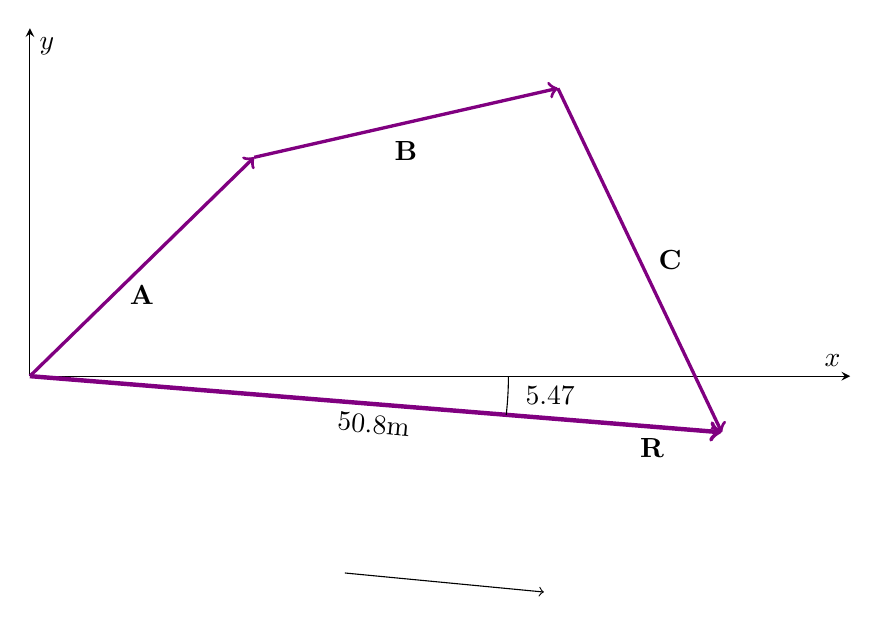
\begin{tikzpicture}
    
        \begin{axis}[width=12cm,height=6cm,
            xmin=0,xmax=60,
            ymin=0,ymax=30,
            axis lines=center,
            ticks=none,
            clip=false,
            ylabel=$y$,
            xlabel=$x$,
            clip=false,
        ]
        \coordinate (A) at ({25*cos(49)},{25*sin(49)});
        \coordinate (B) at ({23*cos(15)},{23*sin(15)});
        \coordinate (AB) at ({25*cos(49)+23*cos(15)},{25*sin(49)+23*sin(15)});
        \coordinate (C) at ({32*cos(-68)},{32*sin(-68)});
        \coordinate (R) at ({50.8*cos(-5.47)},{50.8*sin(-5.47)});
        
        \draw[very thick,violet,->] (0,0) -- (A) node[black,pos=0.5,below=1mm] {$\textbf{A}$};
        \draw[very thick,violet,->] (A) -- ++(B) node[pos=0.5,black,below=1mm] {$\textbf{B}$};
        \draw[very thick,violet,->] (AB) -- ++(C) node[pos=0.5,black,right=1mm] {$\textbf{C}$};
        \draw[ultra thick,violet,->] (0,0) -- (R) node[black,pos=0.5,below,rotate=-5.47] {\SI{50.8}{m}} node[pos=0.9,below,black] {$\textbf{R}$};
        \draw (35,0) arc (0:-5.47:35) node[pos=0.5,right=1mm] {\ang{5.47}};
        \end{axis}
        \tkzRegle[Fond=true,Opacite=0.9,CouleurFond=yellow,AfficheValeurs=false,Origine={(0.2,-0.6)},Echelle=0.6,Rotation=-5.47]
        \tkzRapporteur[Fond,CouleurFond=blue,Echelle=0.4,Origine={(4,-2.5)},AfficheAngles=false,Rotation=-180]
        \draw[->] (4,-2.5) -- ++ ({0.05*50.8*cos(-5.47)},{0.05*50.8*sin(-5.47)});
    \end{tikzpicture}
\end{center}

In this case, the total displacement $\textbf{R}$ is seen to have a magnitude of \SI{50.8}{m} and to lie in a direction  \ang{5.47} south of east. By using its magnitude and direction, this vector can be expressed as $\textbf{R} = \SI{50.8}{m}$ and $\theta = \ang{5.47}$ south of east.

\vspace{1em}

\textbf{Discussion}: The head-to-tail graphical method of vector addition works for any number of vectors. It is also important to note that the resultant is independent of the order in which the vectors are added. Therefore, we could add the vectors in any order as illustrated in Figure \ref{ondDEl} and we will still get the same solution.

\begin{center}
    \begin{tikzpicture}
        \begin{axis}[width=12cm,height=6cm,
            xmin=0,xmax=60,
            ymin=0,ymax=30,
            axis lines=center,
            ticks=none,
            clip=false,
            ylabel=$y$,
            xlabel=$x$,
            clip=false,
        ]
        \coordinate (A) at ({25*cos(49)},{25*sin(49)});
        \coordinate (B) at ({23*cos(15)},{23*sin(15)});
        \coordinate (AB) at ({25*cos(49)+23*cos(15)},{25*sin(49)+23*sin(15)});
        \coordinate (C) at ({32*cos(-68)},{32*sin(-68)});
        \coordinate (CA) at ({32*cos(-68)+25*cos(49)},{32*sin(-68)+25*sin(49)});
        \coordinate (R) at ({50.8*cos(-5.47)},{50.8*sin(-5.47)});
        
        \draw[very thick,violet,->] (0,0) -- (C) node[black,pos=0.5,below left] {$\textbf{C}$};
        \draw[very thick,violet,->] (C) -- ++(A) node[pos=0.5,black,below right] {$\textbf{A}$};
        \draw[very thick,violet,->] (CA) -- ++(B) node[pos=0.4,black,below right] {$\textbf{B}$};
        \draw[ultra thick,violet,->] (0,0) -- (R) node[black,pos=0.5,below,rotate=-5.47] {\SI{50.8}{m}} node[pos=0.9,above,black] {$\textbf{R}$};
        \draw (35,0) arc (0:-5.47:35) node[pos=0.5,right=1mm] {\ang{5.47}};
        \end{axis}
    \end{tikzpicture}
\end{center}

Here, we see that when the same vectors are added in a different order, the result is the same. This characteristic is true in every case and is an important characteristic of vectors. Vector addition is commutative. Vectors can be added in any order.

\begin{equation}
    \textbf{A} + \textbf{B} = \textbf{B} + \textbf{A}
\end{equation}

(This is true for the addition of ordinary numbers as well---you get the same result whether you add $2+3$ or $3+2$, for example).

\endsolution

\subsubsection*{Vector Subtraction}

Vector subtraction is a straightforward extension of vector addition. To define subtraction (say we want to subtract \textbf{B} from  \textbf{A}, written $\textbf{A} - \textbf{B}$) we must first define what we mean by subtraction. The \textit{negative} of a vector \textbf{B} is defined to be $-\textbf{B}$; that is, \textit{graphically the negative of any vector has the same magnitude but the opposite direction}, as shown in Figure \ref{sxiWCS}. In other words,  \textbf{B} has the same length as $-\textbf{B}$, but points in the opposite direction. Essentially, we just flip the vector so it points in the opposite direction.

\begin{center}
    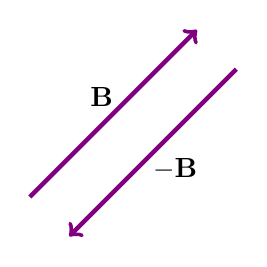
\begin{tikzpicture}
        \draw[ultra thick,violet,->] (0,0) -- ({3*cos(45)},{3*sin(45)}) node[right,pos=0.6,left=2pt,black] {\textbf{B}};
        \begin{scope}[shift={(0.5,-0.5)}]
            \draw[ultra thick,violet,<-] (0,0) -- ({3*cos(45)},{3*sin(45)}) node[right,pos=0.4,right=2pt,black] {$-\textbf{B}$};
        \end{scope}
    \end{tikzpicture}
    \captionsetup{type=figure,margin=1in,font=scriptsize}
    \captionof{figure}{The negative of a vector is just another vector of the same magnitude but pointing in the opposite direction. So \textbf{B} is the negative of $-\textbf{B}$; it has the same length but opposite direction.}
    \label{sxiWCS}
\end{center}

The subtraction of vector \textbf{B} from vector \textbf{A} is then simply defined to be the addition of $-\textbf{B}$ to \textbf{A}. Note that vector subtraction is the addition of a negative vector. The order of subtraction does not affect the results.

\begin{equation}
    \textbf{A} - \textbf{B} = \textbf{A} + \left(-\textbf{B}\right)
\end{equation}

This is analogous to the subtraction of scalars (where, for example,  $5 – 2 = 5 + (–2)$ ). Again, the result is independent of the order in which the subtraction is made. When vectors are subtracted graphically, the techniques outlined above are used, as the following example illustrates.

\begin{example}
    \textit{Subtracting Vectors Graphically: A Woman Sailing a Boat}. A woman sailing a boat at night is following directions to a dock. The instructions read to first sail \SI{27.5}{m} in a direction \ang{66.0} north of east from her current location, and then travel \SI{30.0}{m} in a direction \ang{112} north of east (or \ang{22.0} west of north). If the woman makes a mistake and travels in the opposite direction for the second leg of the trip, where will she end up? Compare this location with the location of the dock.
\end{example}

\begin{center}    
    \begin{tikzpicture}
        \begin{axis}[width=6cm,height=6cm,
            xmin=0,xmax=40,
            ymin=0,ymax=40,
            ticks=none,
            axis lines=none,
            clip=false,
        ]
        \draw[thick,->] (0,0) -- ++(10,0) node[right] {$x$};
        \draw[thick,->] (0,0) -- ++(0,10) node[above] {$y$};
        \end{axis}
    \end{tikzpicture}%
    \hspace{4em}
    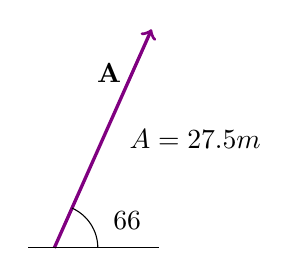
\begin{tikzpicture}
        \begin{axis}[width=6cm,height=6cm,
            xmin=0,xmax=40,
            ymin=0,ymax=40,
            ticks=none,
            axis lines=none,
            clip=false,
        ]
        \coordinate (A) at ({27.5*cos(66)},{27.5*sin(66)});
        \draw[->,very thick, violet] (0,0) -- ++ (A) node[pos=0.8,left,black] {$\textbf{A}$} node[pos=0.5,right=2mm,black] {$A = \SI{27.5}{m}$};
        \draw (-3,0) -- ++(15,0);
        \draw (5,0) arc (0:66:5) node[pos=0.6,right=2mm] {\ang{66}};
        \end{axis}
    \end{tikzpicture}%
    \hspace{2em}
    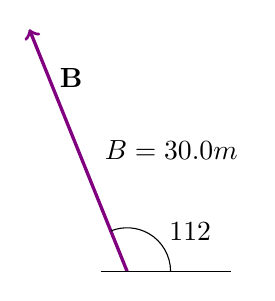
\begin{tikzpicture}
        \begin{axis}[width=6cm,height=6cm,
            xmin=0,xmax=40,
            ymin=0,ymax=40,
            ticks=none,
            axis lines=none,
            clip=false,
        ]
        \coordinate (B) at ({30*cos(112)},{30*sin(112)});
        \draw[->,very thick, violet] (0,0) -- ++ (B) node[pos=0.8,right,black] {$\textbf{B}$} node[black,pos=0.5,right=2mm] {$B = \SI{30.0}{m}$};
        \draw (-3,0) -- ++(15,0);
        \draw (5,0) arc (0:112:5) node[pos=0.6,right=2mm] {\ang{112}};
        \end{axis}
    \end{tikzpicture}
\end{center}

\Solution \textbf{Strategy}: We can represent the first leg of the trip with a vector \textbf{A}, and the second leg of the trip with a vector \textbf{B}. The dock is located at a location $\textbf{A} + \textbf{B}$. If the woman mistakenly travels in the \textit{opposite} direction for the second leg of the journey, she will travel a distance $B$ (\SI{30.0}{m}) in the direction $\ang{180} - \ang{112} = \ang{68}$ south of east. We represent this as $-\textbf{B}$, as shown below. The vector $-\textbf{B}$ has the same magnitude as \textbf{B} but is in the opposite direction. Thus, she will end up at a location $\textbf{A} + \left(-\textbf{B}\right)$, or $\textbf{A} - \textbf{B}$.

\begin{center}
    \begin{tikzpicture}
        \begin{axis}[width=6cm,height=6cm,
            xmin=0,xmax=40,
            ymin=0,ymax=40,
            ticks=none,
            axis lines=none,
            clip=false,
        ]
        \coordinate (nB) at ({30*cos(112-180)},{30*sin(112-180)});
        \draw[->,very thick, violet] (0,0) -- ++ (nB) node[pos=0.8,above right,black] {$-\textbf{B}$};
        \draw (-3,0) -- ++(15,0);
        \draw[violet,dashed,thick] (0,0) -- ({10*cos(112)},{10*sin(112)});
        \draw (3,0) arc (0:112:3) node[pos=0.8,right=2mm] {\ang{112}};
        \draw (6,0) arc (0:-68:6) node[pos=0.8,right=1mm] {\ang{68}};

        \begin{scope}[shift={(-25,0)}]
            \draw[thick,->] (0,0) -- ++(10,0) node[right] {$x$};
            \draw[thick,->] (0,0) -- ++(0,10) node[above] {$y$};
        \end{scope}
        \end{axis}
    \end{tikzpicture}
\end{center}

We will perform vector addition to compare the location of the dock, $\textbf{A} + \textbf{B}$, with the location at which the woman mistakenly arrives, $\textbf{A} + \left(-\textbf{B}\right)$.

\vspace{1em}

(1) To determine the location at which the woman arrives by accident, draw vectors $\textbf{A}$ and $-\textbf{B}$.

\vspace{1em}

(2) Place the vectors head to tail.

\vspace{1em}

(3) Draw the resultant vector \textbf{R}.

\vspace{1em}

(4) Use a ruler and protractor to measure the magnitude and direction of $\textbf{R}$.

\begin{center}
    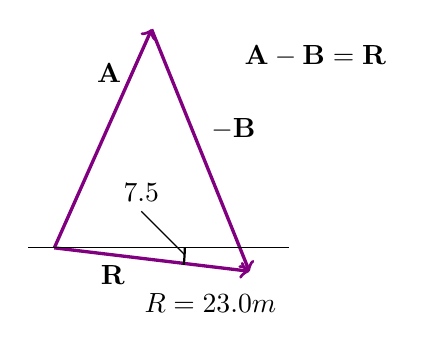
\begin{tikzpicture}
        \begin{axis}[width=6cm,height=6cm,
            xmin=0,xmax=40,
            ymin=0,ymax=40,
            ticks=none,
            axis lines=none,
            clip=false,
        ]
        \coordinate (A) at ({27.5*cos(66)},{27.5*sin(66)});
        \coordinate (nB) at ({30*cos(112-180)},{30*sin(112-180)});
        \coordinate (AnB) at ({27.5*cos(66)+30*cos(112-180)},{27.5*sin(66)+30*sin(112-180)});
        
        \draw[->,very thick, violet] (0,0) -- ++ (A) node[pos=0.8,left,black] {$\textbf{A}$};
        \draw[->,very thick, violet] (A) -- ++(nB) node[pos=0.5,above right,black] {$-\textbf{B}$};
        \draw[->,very thick,violet] (0,0) -- ++ (AnB) node[black,pos=0.3,below] {\textbf{R}} node[pos=0.8,black,below=2mm] {$R = \SI{23.0}{m}$};
        \draw (-3,0) -- ++(30,0);
        \draw[thick] (15,0) arc (0:-7.5:15);
        \draw (15,-0.8) -- ++(-5,5) node[above] {\ang{7.5}};
        \node at (30,22) {$\textbf{A} - \textbf{B} = \textbf{R}$};
        \end{axis}
    \end{tikzpicture}
\end{center}

In this case, $R = \SI{23.0}{m}$ and $\theta = \ang{7.5}$ south of east.

\vspace{1em}

(5) To determine the location of the dock, we repeat this method to add vectors  \textbf{A} and  \textbf{B}. We obtain the resultant vector $\textbf{R}^{\prime}$:

\begin{center}
    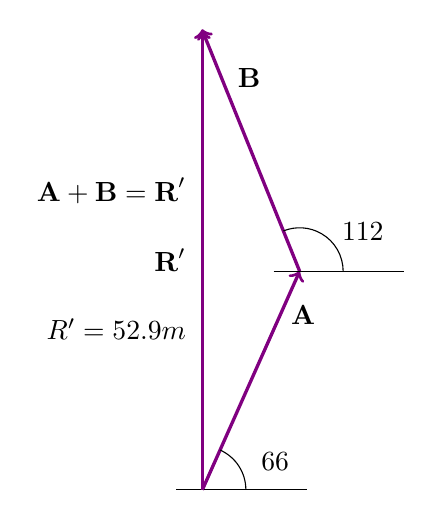
\begin{tikzpicture}
        \begin{axis}[width=6cm,height=6cm,
            xmin=0,xmax=40,
            ymin=0,ymax=40,
            ticks=none,
            axis lines=none,
            clip=false,
        ]
        \coordinate (A) at ({27.5*cos(66)},{27.5*sin(66)});
        \coordinate (B) at ({30*cos(112)},{30*sin(112)});
        \draw[->,very thick, violet] (0,0) -- ++ (A) node[pos=0.8,right,black] {$\textbf{A}$};
        \draw (-3,0) -- ++(15,0);
        \draw (5,0) arc (0:66:5) node[pos=0.6,right=2mm] {\ang{66}};
        \draw[violet,very thick,->] (A) -- ++(B) node[pos=0.8,right=2pt,black] {\textbf{B}};
        \draw ({27.5*cos(66)-3},{27.5*sin(66)}) -- ++(15,0);
        \draw ({27.5*cos(66)+5},{27.5*sin(66)}) arc (0:112:5) node[pos=0.6,right=2mm] {\ang{112}};
        \draw[very thick, violet,->] (0,0) -- ++(0,52.9) node[black,pos=0.5,left=2pt] {$\textbf{R}^{\prime}$} node[black,pos=0.35,left=2pt] {$R^{\prime} = \SI{52.9}{m}$} node[black,left=2pt,pos=0.65] {$\textbf{A} + \textbf{B} = \textbf{R}^{\prime}$};
        \end{axis}
    \end{tikzpicture}
\end{center}

In this case  $R = \SI{52.9}{m}$ and $\theta = \ang{90.1}$ north of east.

\vspace{1em}

We can see that the woman will end up a significant distance from the dock if she travels in the opposite direction for the second leg of the trip.

\vspace{1em}

\textbf{Discussion}: Because subtraction of a vector is the same as addition of a vector with the opposite direction, the graphical method of subtracting vectors works the same as for addition.

\endsolution

\subsubsection*{Multiplication of Vectors and Scalars}

If we decided to walk three times as far on the first leg of the trip considered in the preceding example, then we would walk $3 \times \SI{27.5}{m}$, or \SI{82.5}{m}, in a direction \ang{66.0} north of east. This is an example of multiplying a vector by a positive scalar. Notice that the magnitude changes, but the direction stays the same.

\vspace{1em}

If the scalar is negative, then multiplying a vector by it changes the vector's magnitude and gives the new vector the opposite direction. For example, if you multiply by $–2$, the magnitude doubles but the direction changes. We can summarize these rules in the following way: When vector \textbf{A} is multiplied by a scalar $c$,

\vspace{1ex}

\begin{itemize}
    \item the magnitude of the vector becomes the absolute value of $cA$,
    \item if $c$ is positive, the direction of the vector does not change,
    \item if $c$ is negative, the direction is reversed.
\end{itemize}

In our case,  $c=3$ and  $A = \SI{27.5}{m}$. Vectors are multiplied by scalars in many situations. Note that division is the inverse of multiplication. For example, dividing by 2 is the same as multiplying by the value (1/2). The rules for multiplication of vectors by scalars are the same for division; simply treat the divisor as a scalar between 0 and 1.

\subsubsection*{Resolving a Vector into Components}

In the examples above, we have been adding vectors to determine the resultant vector. In many cases, however, we will need to do the opposite. We will need to take a single vector and find what other vectors added together produce it. In most cases, this involves determining the perpendicular components of a single vector, for example the $x$- and $y$-components, or the north-south and east-west components.

\vspace{1em}

For example, we may know that the total displacement of a person walking in a city is 10.3 blocks in a direction \ang{29.0} north of east and want to find out how many blocks east and north had to be walked. This method is called finding the components (or parts) of the displacement in the east and north directions, and it is the inverse of the process followed to find the total displacement. It is one example of finding the components of a vector. There are many applications in physics where this is a useful thing to do. We will see this soon in Projectile Motion, and much more when we cover forces in ``Dynamics: Newton’s Laws of Motion.'' Most of these involve finding components along perpendicular axes (such as north and east), so that right triangles are involved. The analytical techniques presented in ``Vector Addition and Subtraction: Analytical Methods'' are ideal for finding vector components.

\begin{gradient}{PHET EXPLORATIONS}
    \textbf{Maze Game}: Learn about position, velocity, and acceleration in the ``Arena of Pain''. Use the green arrow to move the ball. Add more walls to the arena to make the game more difficult. Try to make a goal as fast as you can.

    \vspace{1em}

    \href{https://openstax.org/l/28mazegame}{Click to view content}.
\end{gradient}

\subsection{Vector Addition and Subtraction: Analytical Methods}

\Gls{analytical method}s of vector addition and subtraction employ geometry and simple trigonometry rather than the ruler and protractor of graphical methods. Part of the graphical technique is retained, because vectors are still represented by arrows for easy visualization. However, analytical methods are more concise, accurate, and precise than graphical methods, which are limited by the accuracy with which a drawing can be made. Analytical methods are limited only by the accuracy and precision with which physical quantities are known.

\subsubsection*{Resolving a Vector into Perpendicular Components}

Analytical techniques and right triangles go hand-in-hand in physics because (among other things) motions along perpendicular directions are independent. We very often need to separate a vector into perpendicular components. For example, given a vector like \textbf{A} in Figure \ref{WZk9xk}, we may wish to find which two perpendicular vectors,  $\textbf{A}_x$  and $\textbf{A}_y$, add to produce it.


 \begin{center}
    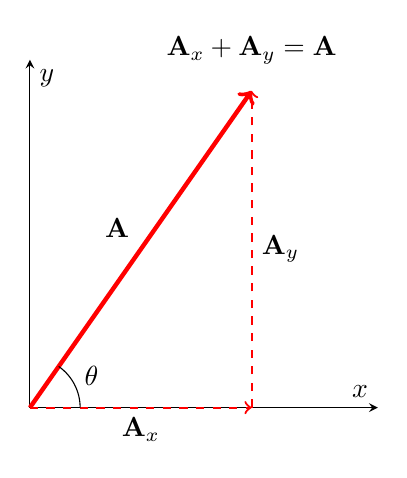
\begin{tikzpicture}
        \begin{axis}[width=6cm,height=6cm,
            axis lines=center,
            xlabel=$x$,
            ylabel=$y$,
            ticks=none,
            xmin=0,xmax=9,
            ymin=0,ymax=9,
            clip=false,            
        ]
        \coordinate (A) at ({10*cos(55)},{10*sin(55)});
        \coordinate (Ax) at ({10*cos(55)},0);
        \coordinate (Ay) at (0,{10*sin(55)});
        
        \draw[ultra thick,red,->] (0,0) -- (A) node[above left,black,pos=0.5] {\textbf{A}} node[above=2mm,black] {$\textbf{A}_x + \textbf{A}_y = \textbf{A}$};
        \node[above left=-6pt] at (Ax) {\Large $\square$};
        \draw[thick,dashed,->,red] (0,0) -- (Ax) node[black,below,pos=0.5] {$\textbf{A}_x$};
        \draw[thick,dashed,->,red] (Ax) -- ++(Ay) node[black,right,pos=0.5] {$\textbf{A}_y$};
        \draw (1.3,0) arc (0:55:1.3) node[right=2pt,pos=0.7] {$\theta$};
        \end{axis}
    \end{tikzpicture}
    \captionsetup{type=figure,margin=1in,font=scriptsize}
    \captionof{figure}{The vector \textbf{A}, with its tail at the origin of an $x$, $y$-coordinate system, is shown together with its $x$- and $y$-components, $\textbf{A}_x$ and $\textbf{A}_y$. These vectors form a right triangle. The analytical relationships among these vectors are summarized below.}
    \label{WZk9xk}
 \end{center}

$\textbf{A}_x$ and $\textbf{A}_y$ are defined to be the components of \textbf{A} along the $x$- and $y$-axes. The three vectors \textbf{A}, $\textbf{A}_x$, and $\textbf{A}_y$ form a right triangle:

\begin{equation}
    \textbf{A}_x + \textbf{A}_y = \textbf{A}
\end{equation}

Note that this relationship between vector components and the resultant vector holds only for vector quantities (which include both magnitude and direction). The relationship does not apply for the magnitudes alone. For example, if  $\textbf{A}_x = \SI{3}{m}$ east, $\textbf{A}_y = \SI{4}{m}$ north, and $\textbf{A}=\SI{5}{m}$ north-east, then it is true that the vectors $\textbf{A}_x + \textbf{A}_y = \textbf{A}$. However, it is \textit{not} true that the sum of the magnitudes of the vectors is also equal. That is,

\begin{equation*}
    \SI{3}{m} + \SI{4}{m} \neq \SI{5}{m}
\end{equation*}

Thus,

\begin{equation*}
    A_x + A_y \neq A
\end{equation*}

If the vector $\textbf{A}$ is known, then its magnitude $A$ (its length) and its angle $\theta$ (its direction) are known. To find $A_x$ and $A_y$, its $x$- and $y$-components, we use the following relationships for a right triangle.

\begin{equation}
    A_x = A \cos{\theta}
\end{equation}

and

\begin{equation}
    A_y = A \sin{\theta}
\end{equation}

\begin{center}
    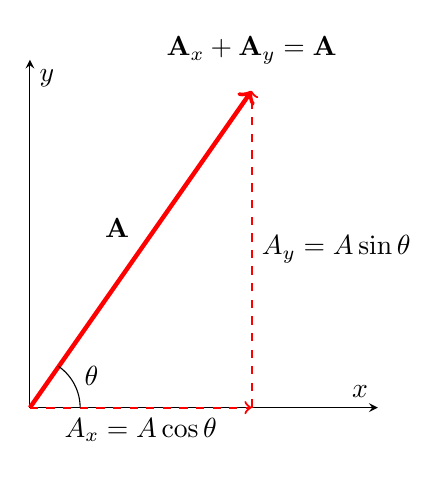
\begin{tikzpicture}
        \begin{axis}[width=6cm,height=6cm,
            axis lines=center,
            xlabel=$x$,
            ylabel=$y$,
            ticks=none,
            xmin=0,xmax=9,
            ymin=0,ymax=9,
            clip=false,            
        ]
        \coordinate (A) at ({10*cos(55)},{10*sin(55)});
        \coordinate (Ax) at ({10*cos(55)},0);
        \coordinate (Ay) at (0,{10*sin(55)});
        
        \draw[ultra thick,red,->] (0,0) -- (A) node[above left,black,pos=0.5] {\textbf{A}} node[above=2mm,black] {$\textbf{A}_x + \textbf{A}_y = \textbf{A}$};
        \node[above left=-6pt] at (Ax) {\Large $\square$};
        \draw[thick,dashed,->,red] (0,0) -- (Ax) node[black,below,pos=0.5] {$A_x = A \cos{\theta}$};
        \draw[thick,dashed,->,red] (Ax) -- ++(Ay) node[black,right,pos=0.5] {$A_y = A \sin{\theta}$};
        \draw (1.3,0) arc (0:55:1.3) node[right=2pt,pos=0.7] {$\theta$};
        \end{axis}
    \end{tikzpicture}
    \captionsetup{type=figure,margin=1in,font=scriptsize}
    \captionof{figure}{The magnitudes of the vector components $\textbf{A}_x$ and  $\textbf{A}_y$ can be related to the resultant vector \textbf{A} and the angle  $\theta$ with trigonometric identities. Here we see that  $A_x = A \cos{\theta}$ and $A_y = A \sin{\theta}$.}
    \label{54hTbj}
 \end{center}

Suppose, for example, that  \textbf{A} is the vector representing the total displacement of the person walking in a city considered in ``Kinematics in Two Dimensions: An Introduction'' and ``Vector Addition and Subtraction: Graphical Methods.''

\begin{center}
    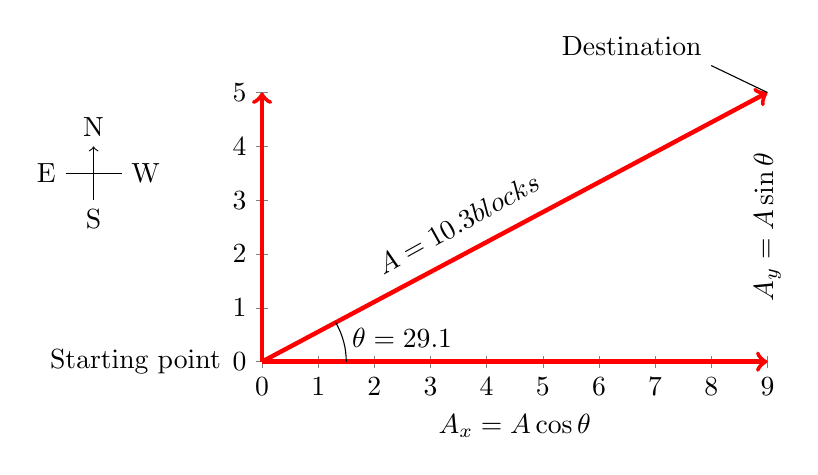
\begin{tikzpicture}
        \begin{axis}[width=8cm, height=5cm,
            xmin=0,xmax=9,
            ymin=0,ymax=5,
            xtick={0,1,...,9},
            ytick={0,1,...,5},
            clip=false,
            axis lines = left,
            xlabel={$A_x = A \cos{\theta}$},
        ]
        \draw[->,ultra thick,red] (0,0) -- (9,0);
        \draw[->,ultra thick,red] (0,0) -- ++(0,5);
        \draw[->,ultra thick,red] (0,0) -- (9,5) node[pos=0.6, above left=1mm,rotate=29,black] {$A = \SI{10.3}{blocks}$};
        \node[left=4mm] at (0,0) {Starting point};
        \draw (9,5) -- ++(-1,0.5) node[above left] {Destination};
        \draw (1.5,0) arc (0:29.1:1.5) node[right,pos=0.6] {$\theta = \ang{29.1}$};
        \node[rotate=90] at (9,2.5) {$A_y = A \sin{\theta}$};
        \begin{scope}[shift={(-3,3)}]
            \draw[->] (0,0) node[below] {S} -- ++(0,1) node[above] {N};
            \draw (-0.5,0.5) node[left] {E} -- ++(1,0) node [right] {W};
        \end{scope}
        \end{axis}
    \end{tikzpicture}
    \captionsetup{type=figure,margin=1in,font=scriptsize}
    \captionof{figure}{We can use the relationships $A_x = A \cos{\theta}$
  and  $A_y = A \sin{\theta}$ to determine the magnitude of the horizontal and vertical component vectors in this example.} 
    \label{b3Ue3i}
\end{center}

Then  $A = \SI{10.3}{blocks}$ and $\theta = \ang{29.1}$, so that

\begin{equation*}
    A_x = A \cos{\theta} = \left(\SI{10.3}{blocks}\right)\left(\cos{\ang{29.1}}\right) = \SI{9.0}{blocks}
\end{equation*}

\begin{equation*}
    A_y = A \sin{\theta} = \left(\SI{10.3}{blocks}\right)\left(\sin{\ang{29.1}}\right) = \SI{5.0}{blocks}
\end{equation*}

\subsubsection*{Calculating a Resultant Vector}

If the perpendicular components  $\textbf{A}_x$ and $\textbf{A}_y$ of a vector \textbf{A} are known, then \textbf{A} can also be found analytically. To find the magnitude $A$ and direction $\theta$ of a vector from its perpendicular components  $\textbf{A}_x$ and $\textbf{A}_y$, relative to the $x$-axis, we use the following relationships:

\begin{equation} \label{oxu9wv}
    A = \sqrt{A_x^2 + A_y^2}
\end{equation}

\begin{equation}
    \theta = \tan^{-1}\left(\frac{A_y}{A_x}\right)
\end{equation}

\begin{center}
    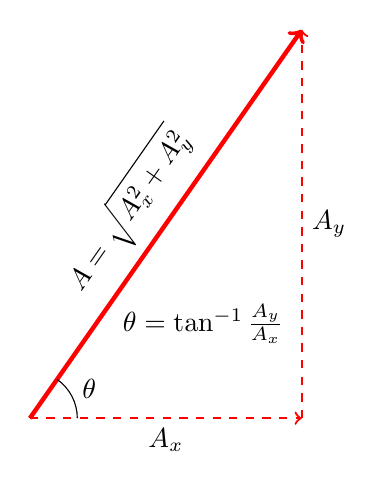
\begin{tikzpicture}
        \begin{axis}[width=7cm,height=7cm,
            axis lines=none,
            xlabel=$x$,
            ylabel=$y$,
            ticks=none,
            xmin=0,xmax=9,
            ymin=0,ymax=9,
            clip=false,            
        ]
        \coordinate (A) at ({10*cos(55)},{10*sin(55)});
        \coordinate (Ax) at ({10*cos(55)},0);
        \coordinate (Ay) at (0,{10*sin(55)});
        
        \draw[ultra thick,red,->] (0,0) -- (A) node[above left,black,pos=0.7,rotate=55] {$A = \sqrt{A_x^2 + A_y^2}$};
        \node[above left=-6pt] at (Ax) {\Large $\square$};
        \draw[thick,dashed,->,red] (0,0) -- (Ax) node[black,below,pos=0.5] {$A_x$};
        \draw[thick,dashed,->,red] (Ax) -- ++(Ay) node[black,right,pos=0.5] {$A_y$};
        \draw (1,0) arc (0:55:1) node[right=2pt,pos=0.7] {$\theta$};
        \end{axis}
        \node at (2.2,1.2) {$\theta = \tan^{-1} \frac{A_y}{A_x}$};
    \end{tikzpicture}
    \captionsetup{type=figure,margin=1in,font=scriptsize}
    \captionof{figure}{The magnitude and direction of the resultant vector can be determined once the horizontal and vertical components $A_x$ and $A_y$ have been determined.}
    \label{IHuUz3}
 \end{center}

 Note that Equation \eqref{oxu9wv} is just the Pythagorean theorem relating the legs of a right triangle to the length of the hypotenuse. For example, if $A_x$ and $A_y$ are 9 and 5 blocks, respectively, then  $A = \sqrt{9^2 + 5^2} = \SI{10.3}{blocks}$, again consistent with the example of the person walking in a city. Finally, the direction is $\theta=\tan^{-1}(5/9) = \ang{29.1}$, as before.

\begin{gradient}{DETERMINING VECTORS AND VECTOR COMPONENTS WITH ANALYTICAL METHODS}
    Equations $A_x = \cos{\theta}$ and  $A_y = \sin{\theta}$ are used to find the perpendicular components of a vector---that is, to go from $A$ and $\theta$ to $A_x$ and $A_y$. Equations $A = \sqrt{A_x^2 + A_y^2}$ and  $\theta = \tan^{-1}(A_y/A_x)$ are used to find a vector from its perpendicular components---that is, to go from $A_x$ and $A_y$ to $A$ and $\theta$. Both processes are crucial to analytical methods of vector addition and subtraction.
\end{gradient}

\subsubsection*{Adding Vectors Using Analytical Methods}

To see how to add vectors using perpendicular components, consider Figure \ref{i2ER22}, in which the vectors \textbf{A} and \textbf{B} are added to produce the resultant \textbf{R}.


\begin{center}
    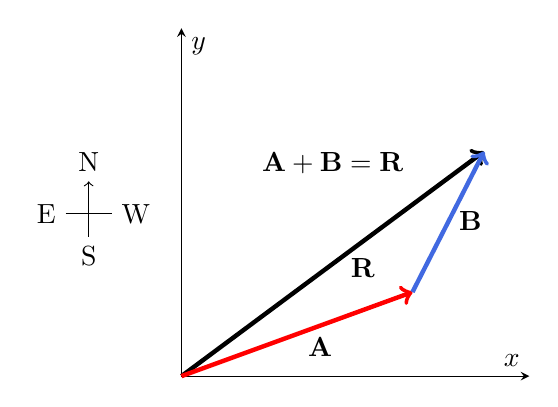
\begin{tikzpicture}
        \begin{axis}[width=6cm,height=6cm,
            axis lines=center,
            xmin=0,xmax=75,
            ymin=0,ymax=75,
            ticks=none,
            clip=false,
            xlabel=$x$,
            ylabel=$y$
        ]
        \coordinate (R) at ({81.2*cos(36.6)},{81.2*sin(36.6)});
        \coordinate (A) at ({53*cos(20)},{53*sin(20)});
        \coordinate (B) at ({34*cos(63)},{34*sin(63)});
        \draw[ultra thick,->] (0,0) -- (R) node[below=2pt,pos=0.6] {\textbf{R}} node[above=1cm,pos=0.5] {$\textbf{A} + \textbf{B} = \textbf{R}$};
        \draw[ultra thick,->,red] (0,0) -- (A) node[below,pos=0.6,black] {\textbf{A}};
        \draw[ultra thick,->,RoyalBlue] (A) -- ++(B) node[below right=-1mm,pos=0.6,black] {\textbf{B}};
        \begin{scope}[shift={(-20,30)}]
            \draw[->] (0,0) node[below] {S} -- ++(0,12) node[above] {N};
            \draw (-5,5) node[left] {E} -- ++(10,0) node [right] {W};
        \end{scope}
        \end{axis}
    \end{tikzpicture}
    \captionsetup{type=figure,margin=1in,font=scriptsize}
    \captionof{figure}{Vectors \textbf{A} and \textbf{B} are two legs of a walk, and \textbf{R} is the resultant or total displacement. You can use analytical methods to determine the magnitude and direction of \textbf{R}.}
    \label{i2ER22}
\end{center}

If \textbf{A} and \textbf{B} represent two legs of a walk (two displacements), then \textbf{R} is the total displacement. The person taking the walk ends up at the tip of \textbf{R}. There are many ways to arrive at the same point. In particular, the person could have walked first in the $x$-direction and then in the $y$-direction. Those paths are the $x$- and $y$-components of the resultant, $\textbf{R}_x$ and $\textbf{R}_y$. If we know $\textbf{R}_x$ and $\textbf{R}_y$, we can find $R$ and $\theta$ using the equations $A = \sqrt{A_x^2 + A_y^2}$ and $\theta = \tan^{-1} (A_y/A_x)$. When you use the analytical method of vector addition, you can determine the components or the magnitude and direction of a vector.

\vspace{1em}

\textbf{Step 1}. \textit{Identify the x- and y-axes that will be used in the problem. Then, find the components of each vector to be added along the chosen perpendicular axes}. Use the equations $A_x = A \cos{\theta}$ and $A_y = A \sin{\theta}$ to find the components. In Figure \ref{0kxQWq}, these components are $A_x$, $A_y$, $B_x$, and $B_y$. The angles that vectors \textbf{A} and \textbf{B} make with the $x$-axis are $\theta_{\text{A}}$ and $\theta_{\text{B}}$, respectively.

\begin{center}
    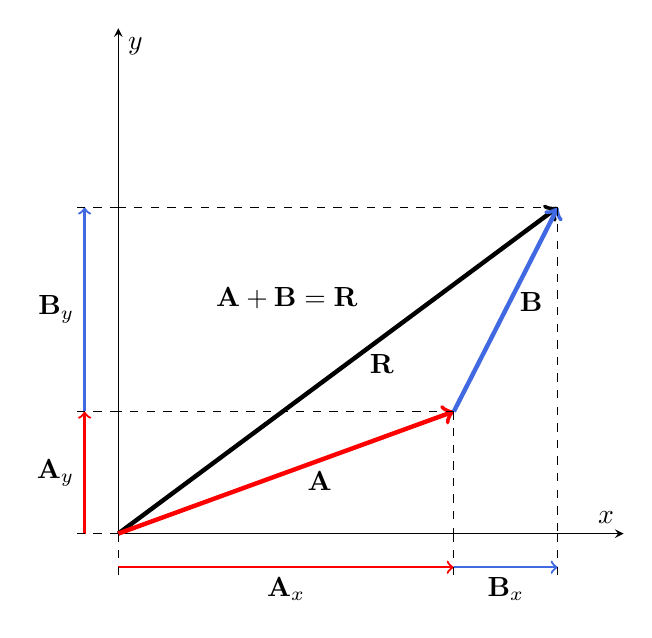
\begin{tikzpicture}
        \begin{axis}[width=8cm,height=8cm,
            axis lines=center,
            xmin=0,xmax=75,
            ymin=0,ymax=75,
            ticks=none,
            clip=false,
            xlabel=$x$,
            ylabel=$y$
        ]
        \coordinate (R) at ({81.2*cos(36.6)},{81.2*sin(36.6)});
        \coordinate (Rx) at ({81.2*cos(36.6)},0);
        \coordinate (A) at ({53*cos(20)},{53*sin(20)});
        \coordinate (Ax) at ({53*cos(20)},0);
        \coordinate (Ay) at (0,{53*sin(20)});
        \coordinate (B) at ({34*cos(63)},{34*sin(63)});
        \coordinate (Bx) at ({34*cos(63)},0);
        \coordinate (By) at (0,{34*sin(63)});
        \draw[ultra thick,->] (0,0) -- (R) node[below=2pt,pos=0.6] {\textbf{R}};
        \node at (25,35) {$\textbf{A} + \textbf{B} = \textbf{R}$};
        \draw[ultra thick,->,red] (0,0) -- (A) node[below,pos=0.6,black] {\textbf{A}};
        \draw[ultra thick,->,RoyalBlue] (A) -- ++(B) node[below right=-1mm,pos=0.6,black] {\textbf{B}};
        
        \draw[dashed] (R) -- ++({-81.2*cos(36.6)},0);
        \draw[dashed] (A) -- ++({-53*cos(20)},0);
        \draw[thick,red,->] (-5,0) -- ++(Ay) node[left,black,pos=0.5] {$\textbf{A}_y$};
        \draw[thick,RoyalBlue,->] (-5,{53*sin(20)}) -- ++(By) node[left,black,pos=0.5] {$\textbf{B}_y$};
        \draw[dashed] (0,{53*sin(20)+34*sin(63)}) -- ++(-7,0);
        \draw[dashed] (0,{53*sin(20)}) -- ++(-7,0);
        \draw[dashed] (0,0) -- ++(-7,0);

        \draw[dashed] (R) -- ++(0,{-81.2*sin(36.6)});
        \draw[dashed] (A) -- ++(0,{-53*sin(20)});
        \draw[thick,red,->] (0,-5) -- ++(Ax) node[below,black,pos=0.5] {$\textbf{A}_x$};
        \draw[thick,RoyalBlue,->] ({53*cos(20)},-5) -- ++(Bx) node[below,black,pos=0.5] {$\textbf{B}_x$};
        \draw[dashed] (0,0) -- ++(0,-7);
        \draw[dashed] ({53*cos(20)+34*cos(63)},0) -- ++(0,-7);
        \draw[dashed] ({53*cos(20)},0) -- ++(0,-7);
        

        % \begin{scope}[shift={(-20,30)}]
        %     \draw[->] (0,0) node[below] {S} -- ++(0,12) node[above] {N};
        %     \draw (-5,5) node[left] {E} -- ++(10,0) node [right] {W};
        % \end{scope}
        \end{axis}
    \end{tikzpicture}
    \captionsetup{type=figure,margin=1in,font=scriptsize}
    \captionof{figure}{To add vectors \textbf{A} and \textbf{B}, first determine the horizontal and vertical components of each vector. These are the dotted vectors $\textbf{A}_x$, $\textbf{A}_y$, $\textbf{B}_x$ and $\textbf{B}_y$ shown in the image.}
    \label{0kxQWq}
\end{center}

\textbf{Step 2}. \textit{Find the components of the resultant along each axis by adding the components of the individual vectors along that axis}. That is, as shown in Figure \ref{QVly9l},

\begin{equation*}
    R_x = A_x + B_x
\end{equation*}

and

\begin{equation*}
    R_y = A_y + B_y
\end{equation*}


\begin{center}
    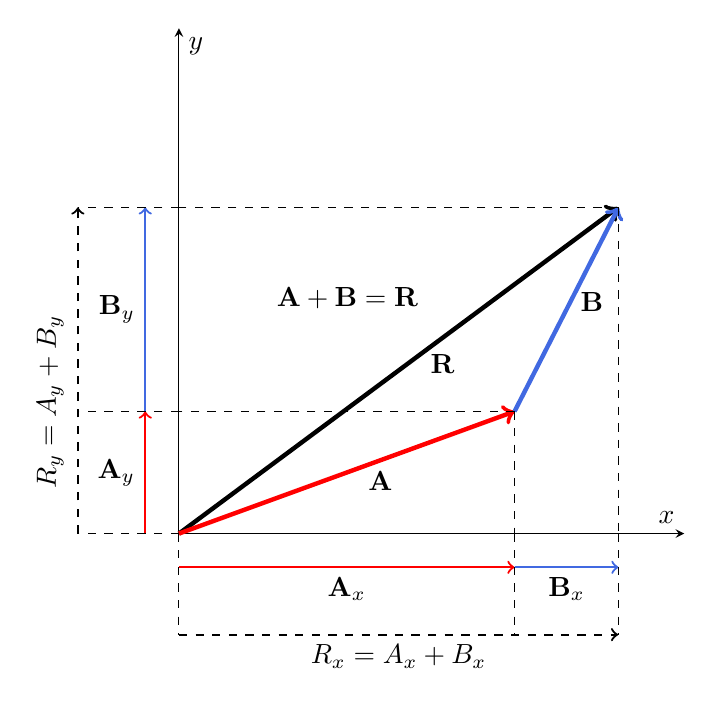
\begin{tikzpicture}
        \begin{axis}[width=8cm,height=8cm,
            axis lines=center,
            xmin=0,xmax=75,
            ymin=0,ymax=75,
            ticks=none,
            clip=false,
            xlabel=$x$,
            ylabel=$y$
        ]
        \coordinate (R) at ({81.2*cos(36.6)},{81.2*sin(36.6)});
        \coordinate (Rx) at ({81.2*cos(36.6)},0);
        \coordinate (Ry) at (0,{81.2*sin(36.6)});
        \coordinate (A) at ({53*cos(20)},{53*sin(20)});
        \coordinate (Ax) at ({53*cos(20)},0);
        \coordinate (Ay) at (0,{53*sin(20)});
        \coordinate (B) at ({34*cos(63)},{34*sin(63)});
        \coordinate (Bx) at ({34*cos(63)},0);
        \coordinate (By) at (0,{34*sin(63)});
        \draw[ultra thick,->] (0,0) -- (R) node[below=2pt,pos=0.6] {\textbf{R}};
        \node at (25,35) {$\textbf{A} + \textbf{B} = \textbf{R}$};
        \draw[ultra thick,->,red] (0,0) -- (A) node[below,pos=0.6,black] {\textbf{A}};
        \draw[ultra thick,->,RoyalBlue] (A) -- ++(B) node[below right=-1mm,pos=0.6,black] {\textbf{B}};
        
        \draw[dashed] (R) -- ++({-81.2*cos(36.6)},0);
        \draw[dashed] (A) -- ++({-53*cos(20)},0);
        \draw[thick,red,->] (-5,0) -- ++(Ay) node[left,black,pos=0.5] {$\textbf{A}_y$};
        \draw[thick,RoyalBlue,->] (-5,{53*sin(20)}) -- ++(By) node[left,black,pos=0.5] {$\textbf{B}_y$};
        \draw[dashed] (0,{53*sin(20)+34*sin(63)}) -- ++(-15,0);
        \draw[dashed] (0,{53*sin(20)}) -- ++(-15,0);
        \draw[dashed] (0,0) -- ++(-15,0);
        
        \draw[thick,dashed,->] (-15,0) -- ++(Ry) node[left=3.5mm,pos=0.7,rotate=90] {$R_y = A_y + B_y$};

        \draw[dashed] (R) -- ++(0,{-81.2*sin(36.6)});
        \draw[dashed] (A) -- ++(0,{-53*sin(20)});
        \draw[thick,red,->] (0,-5) -- ++(Ax) node[below,black,pos=0.5] {$\textbf{A}_x$};
        \draw[thick,RoyalBlue,->] ({53*cos(20)},-5) -- ++(Bx) node[below,black,pos=0.5] {$\textbf{B}_x$};
        \draw[dashed] (0,0) -- ++(0,-15);
        \draw[dashed] ({53*cos(20)+34*cos(63)},0) -- ++(0,-15);
        \draw[dashed] ({53*cos(20)},0) -- ++(0,-15);

        \draw[thick,dashed,->] (0,-15) -- ++(Rx) node[below,pos=0.5] {$R_x = A_x + B_x$};
        \end{axis}
    \end{tikzpicture}
    \captionsetup{type=figure,margin=1in,font=scriptsize}
    \captionof{figure}{The magnitude of the vectors $\textbf{A}_x$ and $\textbf{B}_x$ add to give the magnitude $R_x$ of the resultant vector in the horizontal direction. Similarly, the magnitudes of the vectors $\textbf{A}_y$ and $\textbf{B}_y$ add to give the magnitude $R_y$ of the resultant vector in the vertical direction.}
    \label{QVly9l}
\end{center}

Components along the same axis, say the $x$-axis, are vectors along the same line and, thus, can be added to one another like ordinary numbers. The same is true for components along the $y$-axis. (For example, a 9-block eastward walk could be taken in two legs, the first 3 blocks east and the second 6 blocks east, for a total of 9, because they are along the same direction.) So resolving vectors into components along common axes makes it easier to add them. Now that the components of \textbf{R} are known, its magnitude and direction can be found.

\vspace{1em}

\textbf{Step 3}. \textit{To get the magnitude \textbf{R} of the resultant, use the Pythagorean theorem:}

\begin{equation}
    R = \sqrt{R_x^2 + R_y^2}
\end{equation}

\textbf{Step 4}. \textit{To get the direction of the resultant relative to the $x$-axis:}

\begin{equation}
    \theta = \tan^{-1}\left(\frac{R_y}{R_x}\right)
\end{equation}

The following example illustrates this technique for adding vectors using perpendicular components.

\begin{example}
    \textit{Adding Vectors Using Analytical Methods}\\
    Add the vector \textbf{A} to the vector \textbf{B} shown in Figure \ref{cBsaWa}, using perpendicular components along the $x$- and $y$-axes. The $x$- and $y$-axes are along the east–west and north–south directions, respectively. Vector \textbf{A} represents the first leg of a walk in which a person walks \SI{53.0}{m} in a direction \ang{20.0} north of east. Vector \textbf{B} represents the second leg, a displacement of \SI{34.0}{m} in a direction \ang{63.0} north of east.
\end{example}

\begin{center}
    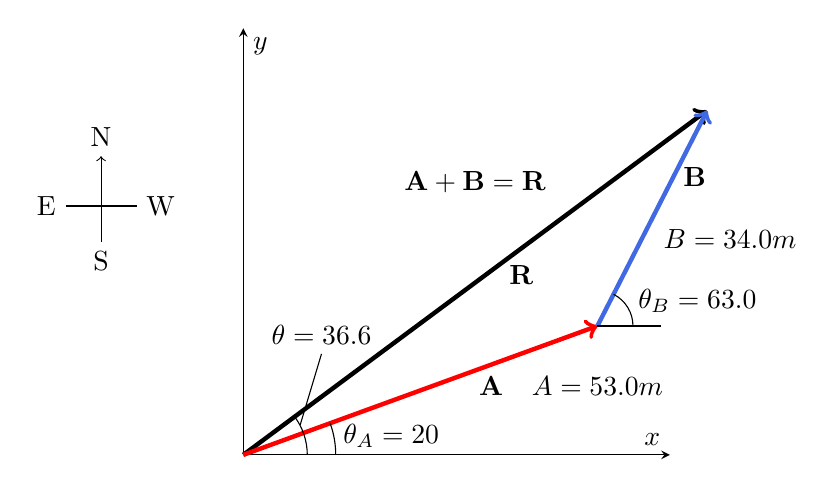
\begin{tikzpicture}
        \begin{axis}[width=7cm,height=7cm,
            axis lines=center,
            xmin=0,xmax=60,
            ymin=0,ymax=60,
            ticks=none,
            clip=false,
            xlabel=$x$,
            ylabel=$y$
        ]
        \coordinate (R) at ({81.2*cos(36.6)},{81.2*sin(36.6)});
        \coordinate (A) at ({53*cos(20)},{53*sin(20)});
        \coordinate (B) at ({34*cos(63)},{34*sin(63)});
        \draw[ultra thick,->] (0,0) -- (R) node[below=2pt,pos=0.6] {\textbf{R}} node[above=1cm,pos=0.5] {$\textbf{A} + \textbf{B} = \textbf{R}$};
        \draw[ultra thick,->,red] (0,0) -- (A) node[below,pos=0.7,black] {\textbf{A}} node[below=5mm,black] {$A = \SI{53.0}{m}$};
        \draw[ultra thick,->,RoyalBlue] (A) -- ++(B) node[below right=-1mm,pos=0.75,black] {\textbf{B}} node[below right,pos=0.5,black] {$B = \SI{34.0}{m}$};
        \draw (9,0) arc (0:36.6:9);
        \draw (13,0) arc (0:20:13) node[right,pos=0.6] {$\theta_{\text{A}} = \ang{20}$};
        \draw (8,4.2) -- ++(3,10) node[above] {$\theta = \ang{36.6}$};
        \begin{scope}[shift={(-20,30)}]
            \draw[->] (0,0) node[below] {S} -- ++(0,12) node[above] {N};
            \draw (-5,5) node[left] {E} -- ++(10,0) node [right] {W};
        \end{scope}
        \draw (A) -- ++(9,0);
        \draw ({53*cos(20) + 5},{53*sin(20)}) arc (0:63:5) node[right=2pt,pos=0.7] {$\theta_{\text{B}} = \ang{63.0}$};
        \end{axis}
    \end{tikzpicture}
    \captionsetup{type=figure,margin=1in,font=scriptsize}
    \captionof{figure}{Vector \textbf{A} has magnitude \SI{53.0}{m} and direction \ang{20.0} north of the $x$-axis. Vector \textbf{B} has magnitude \SI{34.0}{m} and direction \ang{63.0} north of the $x$-axis. You can use analytical methods to determine the magnitude and direction of \textbf{R}.}
\label{cBsaWa}
\end{center}

\Solution \textbf{Strategy}: The components of \textbf{A} and \textbf{B} along the $x$- and $y$-axes represent walking due east and due north to get to the same ending point. Once found, they are combined to produce the resultant.

\vspace{1em}

Following the method outlined above, we first find the components of \textbf{A} and \textbf{B} along the $x$- and $y$-axes. Note that $A = \SI{53.0}{m}$, $\theta_{\text{A}} = \ang{20.0}$, $B = \SI{34.0}{m}$, and $\theta_{\text{B}} = \ang{63.0}$. We find the $x$-components by using $A_x = A \cos{\theta}$, which gives

\begin{equation*}
    A_x = A \cos{\theta_{\text{A}}} = \left(\SI{53.0}{m}\right) \left(\cos{\ang{20.0}}\right) = \left(\SI{53.0}{m}\right) \left(0.940\right) = \SI{49.8}{m}
\end{equation*}

and

\begin{equation*}
    B_x = B\cos{\theta_{\text{B}}} = \left(\SI{34.0}{m}\right) \left(\cos{\ang{63.0}}\right) = \left(\SI{34.0}{m}\right) \left(0.454\right) = \SI{15.4}{m}
\end{equation*}

Similarly, the $y$-components are found using $A_y = A \sin{\theta_{\text{A}}}$:

\begin{equation*}
    A_y = A \sin{\theta_{\text{A}}} = \left(\SI{53.0}{m}\right) \left(\sin{\ang{20.0}}\right) = \left(\SI{53.0}{m}\right) \left(0.342\right) = \SI{18.1}{m}
\end{equation*}

and

\begin{equation*}
    B_y = B\cos{\theta_{\text{B}}} = \left(\SI{34.0}{m}\right) \left(\sin{\ang{63.0}}\right) = \left(\SI{34.0}{m}\right) \left(0.891\right) = \SI{30.3}{m}
\end{equation*}

The $x$- and $y$-components of the resultant are thus

\begin{equation*}
    R_x = A_x + B_x = \SI{49.8}{m} + \SI{15.4}{m} = \SI{65.2}{m}
\end{equation*}

and 

\begin{equation*}
    R_y = A_y + B_y = \SI{18.1}{m} + \SI{30.3}{m} = \SI{48.4}{m}
\end{equation*}

Now we can find the magnitude of the resultant by using the Pythagorean theorem:

\begin{equation*}
    R = \sqrt{R_x^2 + R_y^2} = \sqrt{\left(\SI{65.2}{m}\right)^2 + \left(\SI{48.4}{m}\right)^2} = 
\end{equation*}

so that 

\begin{equation*}
    R = \SI{81.2}{m}
\end{equation*}

Finally, we find the direction of the resultant:

\begin{equation*}
    \theta = \tan^{-1}\left(\frac{R_y}{R_x}\right) = \tan^{-1}\left(\frac{48.4}{65.2}\right) 
\end{equation*}

Thus,

\begin{equation*}
    \theta = \tan^{-1}\left(0.742\right) = \ang{36.6}
\end{equation*}

\begin{center}
    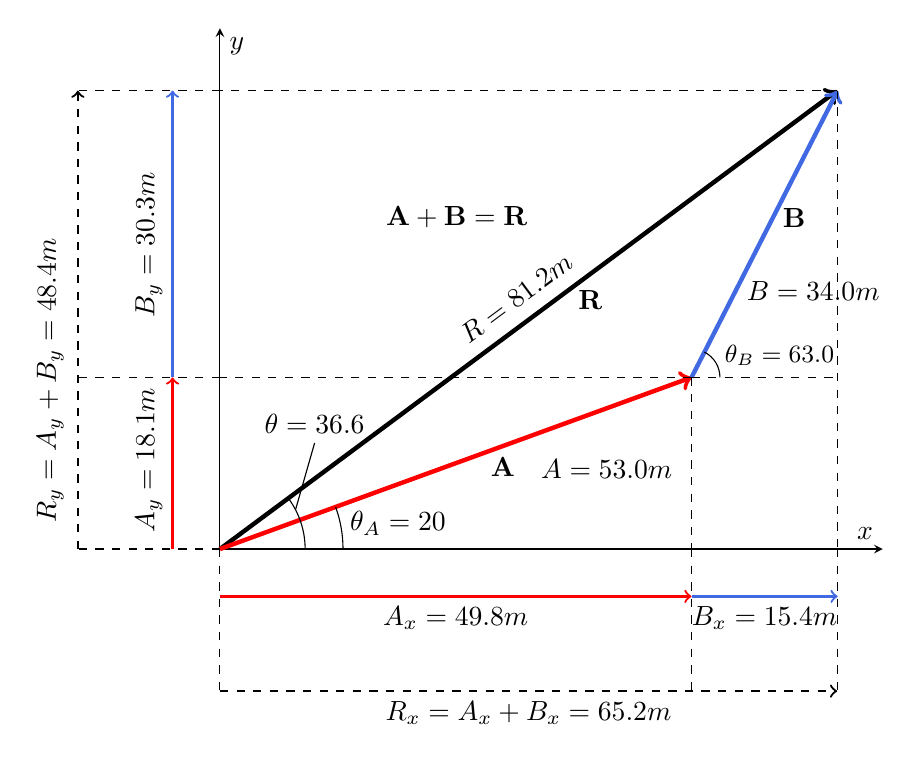
\begin{tikzpicture}
        \begin{axis}[width=10cm,height=10cm,
            axis lines=center,
            xmin=0,xmax=70,
            ymin=0,ymax=55,
            ticks=none,
            clip=false,
            xlabel=$x$,
            ylabel=$y$,
            axis equal image
        ]
        \coordinate (R) at ({81.2*cos(36.6)},{81.2*sin(36.6)});
        \coordinate (Rx) at ({81.2*cos(36.6)},0);
        \coordinate (Ry) at (0,{81.2*sin(36.6)});
        \coordinate (A) at ({53*cos(20)},{53*sin(20)});
        \coordinate (Ax) at ({53*cos(20)},0);
        \coordinate (Ay) at (0,{53*sin(20)});
        \coordinate (B) at ({34*cos(63)},{34*sin(63)});
        \coordinate (Bx) at ({34*cos(63)},0);
        \coordinate (By) at (0,{34*sin(63)});
        
        \draw[ultra thick,->] (0,0) -- (R) node[below=2pt,pos=0.6] {\textbf{R}} node[above=2pt,pos=0.5,rotate=36.6] {$R = \SI{81.2}{m}$};
        \node at (25,35) {$\textbf{A} + \textbf{B} = \textbf{R}$};
        \draw[ultra thick,->,red] (0,0) -- (A) node[below,pos=0.6,black] {\textbf{A}} node[below=5mm,black,pos=0.82] {$A = \SI{53.0}{m}$};
        \draw[ultra thick,->,RoyalBlue] (A) -- ++(B) node[below right=-1mm,pos=0.6,black] {\textbf{B}} node[right,pos=0.3,black] {$B = \SI{34.0}{m}$};
        
        \draw[dashed] (R) -- ++({-81.2*cos(36.6)},0);
        \draw[dashed] (A) -- ++({-53*cos(20)},0);
        \draw[thick,red,->] (-5,0) -- ++(Ay) node[left=3mm,black,rotate=90] {$A_y = \SI{18.1}{m}$};
        \draw[thick,RoyalBlue,->] (-5,{53*sin(20)}) -- ++(By) node[left=3mm,pos=0.75,black,rotate=90] {$B_y = \SI{30.3}{m}$};
        \draw[dashed] (0,{53*sin(20)+34*sin(63)}) -- ++(-15,0);
        \draw[dashed] (0,{53*sin(20)}) -- ++(-15,0);
        \draw[dashed] (0,0) -- ++(-15,0);
        
        \draw[thick,dashed,->] (-15,0) -- ++(Ry) node[left=3.5mm,pos=0.7,rotate=90] {$R_y = A_y + B_y = \SI{48.4}{m}$};
        
        \draw[dashed] (R) -- ++(0,{-81.2*sin(36.6)});
        \draw[dashed] (A) -- ++(0,{-53*sin(20)});
        \draw[thick,red,->] (0,-5) -- ++(Ax) node[below,black,pos=0.5] {$A_x = \SI{49.8}{m}$};
        \draw[thick,RoyalBlue,->] ({53*cos(20)},-5) -- ++(Bx) node[below,black,pos=0.5] {$B_x = \SI{15.4}{m}$};
        \draw[dashed] (0,0) -- ++(0,-15);
        \draw[dashed] ({53*cos(20)+34*cos(63)},0) -- ++(0,-15);
        \draw[dashed] ({53*cos(20)},0) -- ++(0,-15);
        \draw[thick,dashed,->] (0,-15) -- ++(Rx) node[below,pos=0.5] {$R_x = A_x + B_x = \SI{65.2}{m}$};
        \draw (9,0) arc (0:36.6:9);
        \draw (13,0) arc (0:20:13) node[right,pos=0.6] {$\theta_{\text{A}} = \ang{20}$};
        \draw (8,4.2) -- ++(2,7) node[above] {$\theta = \ang{36.6}$};

        \draw[dashed] (A) -- ++(Bx);
        \draw ({53*cos(20) + 3},{53*sin(20)}) arc (0:63:3) node[right=2pt,pos=0.8] {\small $\theta_{\text{B}} = \ang{63.0}$};
        \end{axis}
    \end{tikzpicture}
    \captionsetup{type=figure,margin=1in,font=scriptsize}
    \captionof{figure}{Using analytical methods, we see that the magnitude of \textbf{R} is \SI{81.2}{m} and its direction is \ang{36.6} north of east.}
    \label{QVly9l}
\end{center}

\textbf{Discussion}: This example illustrates the addition of vectors using perpendicular components. Vector subtraction using perpendicular components is very similar--it is just the addition of a negative vector.

\vspace{1em}

Subtraction of vectors is accomplished by the addition of a negative vector. That is, $\textbf{A}-\textbf{B} \equiv \textbf{A}+\left(-\textbf{B}\right)$. Thus, \textit{the method for the subtraction of vectors using perpendicular components is identical to that for addition}. The components of $-\textbf{B}$ are the negatives of the components of \textbf{B}. The $x$- and $y$-components of the resultant  $\textbf{A} - \textbf{B} = \textbf{R}$ are thus

\begin{equation*}
    R_x = A_x + \left(-B_x\right)
\end{equation*}

\begin{equation*}
    R_y = A_y + \left(-B_y\right)
\end{equation*}

and the rest of the method outlined above is identical to that for addition. (See Figure \ref{g2pI0f}.)

\endsolution    

Analyzing vectors using perpendicular components is very useful in many areas of physics, because perpendicular quantities are often independent of one another. The next module, ``Projectile Motion,'' is one of many in which using perpendicular components helps make the picture clear and simplifies the physics.

\begin{center}
    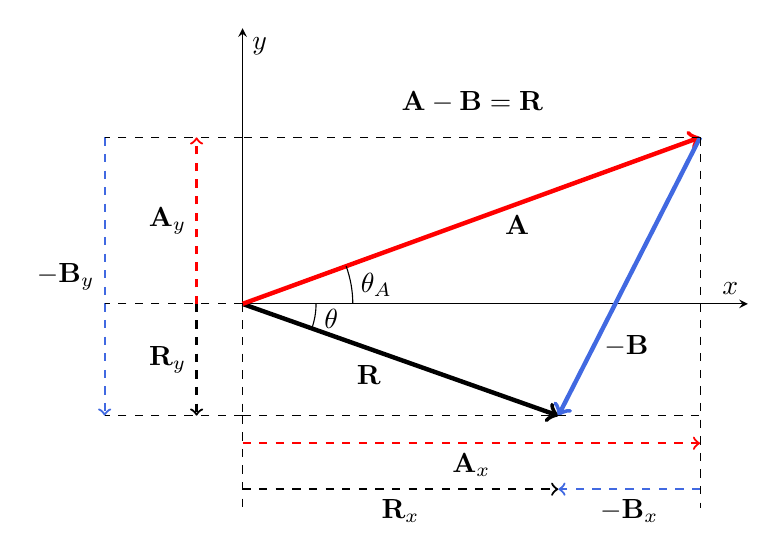
\begin{tikzpicture}
        \begin{axis}[width=8cm,height=8cm,
            axis lines=center,
            xmin=0,xmax=55,
            ymin=0,ymax=30,
            ticks=none,
            clip=false,
            xlabel=$x$,
            ylabel=$y$,
            axis equal image
        ]
        \coordinate (A) at ({53*cos(20)},{53*sin(20)});
        \coordinate (Ax) at ({53*cos(20)},0);
        \coordinate (Ay) at (0,{53*sin(20)});
        \coordinate (B) at ({-34*cos(63)},{-34*sin(63)});
        \coordinate (Bx) at ({-34*cos(63)},0);
        \coordinate (By) at (0,{-34*sin(63)});
        \coordinate (R) at ({53*cos(20)-34*cos(63)},{53*sin(20)-34*sin(63)});
        \coordinate (Ry) at (0,{53*sin(20)-34*sin(63)});
        \coordinate (Rx) at ({53*cos(20)-34*cos(63)},0);
        
        \draw[ultra thick,->] (0,0) -- (R) node[below=2pt,pos=0.4] {\textbf{R}};
        \node at (25,22) {$\textbf{A} - \textbf{B} = \textbf{R}$};
        \draw[ultra thick,->,red] (0,0) -- (A) node[below,pos=0.6,black] {\textbf{A}};
        \draw[ultra thick,->,RoyalBlue] (A) -- ++(B) node[below right=-1mm,pos=0.7,black] {$-\textbf{B}$};
        
        \draw[dashed] (A) -- ++({-53*cos(20)},0);
        
        \draw[thick,dashed,red,->] (-5,0) -- ++(Ay) node[left,black,pos=0.5] {$\textbf{A}_y$};
        \draw[thick,dashed,RoyalBlue,->] (-15,{53*sin(20)}) -- ++(By) node[left,pos=0.5,black] {$-\textbf{B}_y$};
        \draw[thick,dashed,->] (-5,0) -- ++(Ry) node[left,pos=0.5] {$\textbf{R}_y$};

        \draw[dashed] (Ay) -- ++(-15,0);
        \draw[dashed] (A) -- ++(By) -- ++(0,-10);
        \draw[dashed] (0,0) -- ++(Ry);
        \draw[dashed] (Ry) -- ++(-15,0);
        \draw[dashed] (Ry) -- ++(Ax);
        \draw[dashed] (0,0) -- ++(-15,0);
        \draw[dashed] (Ry) -- ++(0,-10);
        \draw[red,thick,dashed,->] (0,{53*sin(20)-34*sin(63)-3}) -- ++(Ax) node[pos=0.5,black,below] {$\textbf{A}_x$};
        \draw[thick,dashed,->] (0,{53*sin(20)-34*sin(63)-8}) -- ++(Rx) node[below,pos=0.5] {$\textbf{R}_x$};
        \draw[thick,RoyalBlue,dashed,->] ({53*cos(20)},{53*sin(20)-34*sin(63)-8}) -- ++(Bx) node[below,pos=0.5,black] {$-\textbf{B}_x$};

        \draw (8,0) arc (0:-19.5:8) node[right,pos=0.6] {$\theta$};
        \draw (12,0) arc (0:20:12) node[right,pos=0.5] {$\theta_{\text{A}}$};
        
        \end{axis}
    \end{tikzpicture}
    \captionsetup{type=figure,margin=1in,font=scriptsize}
    \captionof{figure}{The subtraction of the two vectors shown in Figure \ref{i2ER22}. The components of $-\textbf{B}$ are the negatives of the components of \textbf{B}. The method of subtraction is the same as that for addition.}
    \label{g2pI0f}
\end{center}

\begin{gradient}{PHET EXPLORATIONS}
    \textbf{Vector Addition}: Learn how to add vectors. Drag vectors onto a graph, change their length and angle, and sum them together. The magnitude, angle, and components of each vector can be displayed in several formats.

    \vspace{1em}

    \href{https://phet.colorado.edu/sims/html/vector-addition/latest/vector-addition_all.html}{Click to view content}.
\end{gradient}

\subsection{Projectile Motion}

\Gls{projectile motion} is the \gls{motion} of an object thrown or projected into the air, subject to only the acceleration of gravity. The object is called a \gls{projectile}, and its path is called its \gls{trajectory}. The motion of falling objects, as covered in ``Problem-Solving Basics for One-Dimensional Kinematics,'' is a simple one-dimensional type of projectile motion in which there is no horizontal movement. In this section, we consider two-dimensional projectile motion, such as that of a football or other object for which \gls{air resistance} is negligible.

\vspace{1em}

The most important fact to remember here is that \textit{motions along perpendicular axes are independent} and thus can be analyzed separately. This fact was discussed in ``Kinematics in Two Dimensions: An Introduction,'' where vertical and horizontal motions were seen to be independent. The key to analyzing two-dimensional projectile motion is to break it into two motions, one along the horizontal axis and the other along the vertical. (This choice of axes is the most sensible, because acceleration due to gravity is vertical---thus, there will be no acceleration along the horizontal axis when air resistance is negligible.) As is customary, we call the horizontal axis the x-axis and the vertical axis the y-axis. Figure \ref{vbEBfp} illustrates the notation for displacement, where \textbf{s} is defined to be the total displacement and \textbf{x} and \textbf{y} are its components along the horizontal and vertical axes, respectively. The magnitudes of these vectors are $s$, $x$, and $y$. (Note that in the last section we used the notation \textbf{A} to represent a vector with components $\textbf{A}_x$ and $\textbf{A}_y$. If we continued this format, we would call displacement \textbf{s} with components $\textbf{s}_x$ and $\textbf{s}_y$. However, to simplify the notation, we will simply represent the component vectors as \textbf{x} and \textbf{y}.)

\vspace{1em}

Of course, to describe motion we must deal with velocity and acceleration, as well as with displacement. We must find their components along the $x$- and $y$-axes, too. We will assume all forces except gravity (such as air resistance and friction, for example) are negligible. The components of acceleration are then very simple: $a_y = -g = -\SI{9.80}{m/s^2}$. (Note that this definition assumes that the upwards direction is defined as the positive direction. If you arrange the coordinate system instead such that the downwards direction is positive, then acceleration due to gravity takes a positive value.) Because gravity is vertical, $a_x = 0$. Both accelerations are constant, so the kinematic equations can be used.

\begin{gradient}{REVIEW OF KINEMATIC EQUATIONS (CONSTANT $a$)}
\vspace{-1em}
    \begin{align}
        x &= x_0 + \bar{v} t \\[1ex]
        \bar{v} &= \frac{v_0 + v}{2} \\[1ex]
        v &= v_0 + a t \\[1ex]
        x &= x_0 + v_0 t + \frac{1}{2} a t^2 \\[1ex]
        v^2 &= v_0^2 + 2 a \left(x - x_0\right)
    \end{align}
\vspace{-1em}
\end{gradient}



\begin{center}
    \begin{tikzpicture} 
        \begin{axis}[width=8cm,height=8cm,ticks=none,
            axis lines = center,
            clip=false,
            ylabel = $y$,
            xlabel = $x$,
            xmin=0, xmax=20,
            ymin=0, ymax=16,
            axis equal image
        ]
        \node at (15.6,0.35) {$\square$};
        \draw[red,domain=0:16,variable=\x,samples=200] plot ({\x},{patheq(\x,0,18,70)}) node[above left=-4pt,black] {\faSoccerBallO};
        \draw[->,ultra thick,violet] (0,0) -- ++(16,{patheq(16,0,18,70)}) node[pos=0.5,above=3pt,black]{\textbf{s}};
        \draw[->,dashed,thick,violet] (0,0) -- ++(16,0) node[pos=0.5,below] {\textbf{x}};
        \draw[->,dashed,thick,violet] (16,0) -- ++(0,{patheq(16,0,18,70)}) node[pos=0.5,right] {\textbf{y}};
        % \node at (2.5,0.65) {$\theta$};
        \draw (2,0) arc (0:35:2) node[right=2pt,pos=0.7] {$\theta$}; 
        \draw (0,0) node[left] {\Strichmaxerl[3]};
        \end{axis}
    \end{tikzpicture}
    \captionsetup{type=figure,margin=1in,font=scriptsize}
    \captionof{figure}{The total displacement \textbf{s} of a soccer ball at a point along its path. The vector \textbf{s} has components \textbf{x} and \textbf{y} along the horizontal and vertical axes. Its magnitude is $s$, and it makes an angle $\theta$ with the horizontal.}
    \label{vbEBfp}
\end{center}

Given these assumptions, the following steps are then used to analyze projectile motion:

\vspace{1em}

\textbf{Step 1}. \textit{Resolve or break the motion into horizontal and vertical components along the $x$- and $y$-axes.} These axes are perpendicular, so $A_x = A \cos{\theta}$ and $A_y = A \sin{\theta}$ are used. The magnitude of the components of displacement \textbf{s} along these axes are $x$ and $y$. The magnitudes of the components of the velocity \textbf{v} are $v_x = v \cos{\theta}$ and $v_y = \sin{\theta}$, where $v$ is the magnitude of the velocity and $\theta$ is its direction, as shown in Figure \ref{JdmgME}. Initial values are denoted with a subscript 0, as usual.

\vspace{1em}

\textbf{Step 2}. \textit{Treat the motion as two independent one-dimensional motions, one horizontal and the other vertical}. The kinematic equations for horizontal and vertical motion take the following forms:

\begin{center}
    \textbf{Horizontal Motion}
\end{center}

\vspace{-1em}

\begin{align}
    a_x &= 0 \\[1ex]
    x &= x_0 + v_x t \\[1ex]
    v_x &= v_{0x} = \text{velocity is a constant} \\[1ex]
\end{align}

\begin{center}
    \textbf{Vertical Motion}
\end{center}

\vspace{-1em}

\begin{align}
    a_y &= -g = -\SI{9.80}{m/s^2} \\[1ex]
    y &= y_0 + \frac{1}{2} \left(v_{0y} + v_y\right) t \\[1ex]
    v_y &= v_{0y} - gt \\[1ex]
    y &= y_0 + v_{0y} t - \frac{1}{2} g t^2 \\[1ex]
    v_y^2 &= v_{0y}^2 - 2 g \left(y - y_0\right)
\end{align}

\textbf{Step 3}. \textit{Solve for the unknowns in the two separate motions---one horizontal and one vertical}. Note that the only common variable between the motions is time $t$. The problem solving procedures here are the same as for one-dimensional \gls{kinematics} and are illustrated in the solved examples below.

\vspace{1em}

\textbf{Step 4}. Recombine the two motions to find the total displacement \textbf{s} and velocity \textbf{v}. Because the $x$- and $y$-motions are perpendicular, we determine these vectors by using the techniques outlined in the ``Vector Addition and Subtraction: Analytical Methods'' and employing $A = \sqrt{A_x^2 + A_y^2}$ and  $\theta = \tan^{-1} \left(A_y/A_x\right)$ in the following form, where $\theta$ is the direction of the displacement \textbf{s} and $\theta_{\text{v}}$ is the direction of the velocity \textbf{v}:

\vspace{1em}

\textbf{Total displacement and velocity}

\begin{align}
    s &= \sqrt{x^2 + y^2} \\[1ex]
    \theta &= \tan^{-1} \left(\frac{y}{x}\right) \\[1ex]
    v &= \sqrt{v_x^2 + v_y^2} \\[1ex]
    \theta_{\text{v}} &= \tan^{-1} \left(\frac{v_y}{v_x}\right)
\end{align}

\begin{center}
    \begin{tikzpicture}[declare function={t(\x)=\x/(\vi*cos(\thetai));}]
    \tikzmath{
        \grav = 10;
        \vi = 20;
        \yi = 0;
        \thetai = 45.0;
        \viy = \vi*sin(\thetai);
        \ymax = (\viy^2)/(2*\grav);
        \tmax = 2*\ymax/\viy;
        \vix = \vi*cos(\thetai);
        \xmax = \vix*\tmax;
        \sf = 0.3; %scale factor for vector components
    }
    % \pgfplotsset{compat=1.11}
        \begin{axis}[width=16cm,ticks=none,
        axis lines = none,
        clip=false,
        ylabel = $y$,
        xlabel = $x$,
        xmin=0, xmax=50,
        ymin=0, ymax=15,
        ]
        \draw[gray,->] (0,0) -- ++(0,10) node[right] {$y$};
        \draw[gray,->] (0,0) -- ++(48,0) node[above] {$x$};
        \draw[fill=black] (0,0) circle (2pt);
        \draw[thick,violet,->] (0,0) -- ++(\vix*\sf,\viy*\sf) node[below right] {$v_0$};
        \draw[thick,dashed,red,->] (0,0) -- ++(0,{\sf*\vi*sin(\thetai)}) node[right=-2pt] {$v_{0y}$};
        \draw[thick,dashed,RoyalBlue,->] (0,0) -- ++(\vix*\sf,0) node[pos=1.3, above=-2pt] {$v_{0x}$};
        \draw (1,0) arc (0:75:0.6) node[midway,right=-1pt] {$\theta_0$};
        
        \pgfplotsinvokeforeach{5,10,15}{
                \draw[fill=black] (#1,{patheqten(#1,0,20,45)}) circle (2pt);
                \draw[thick,dashed,red,->] (#1,{patheqten(#1,0,20,45)}) -- ++(0,{\sf*(\vi*sin(\thetai) - \grav*t(#1))}) node[above=-2pt] {$v_y$};
                \draw[thick,dashed,RoyalBlue,->] (#1,{patheqten(#1,0,20,45)}) -- ++(\vix*\sf,0) node[right=-2pt] {$v_x$};
                \draw[thick,violet,->] (#1,{patheqten(#1,0,20,45)}) -- ++(\vix*\sf,{\sf*(\vi*sin(\thetai) - \grav*t(#1))}) node[above=-2pt] {$v$};
                }
                
        \draw[fill=black] (\xmax,\ymax) circle (2pt);
        \draw[thick,violet,->] (\xmax,\ymax) -- ++(\vix*\sf,0) node[right=-2pt] {$v = v_x$};
        
        \pgfplotsinvokeforeach{25,30,35,45}{
                \draw[fill=black] (#1,{patheqten(#1,0,20,45)}) circle (2pt);
                \draw[thick,dashed,red,->] (#1,{patheqten(#1,0,20,45)}) -- ++(0,{\sf*(\vi*sin(\thetai) - \grav*t(#1))}) node[below=-2pt] {$v_y$};
                \draw[thick,dashed,RoyalBlue,->] (#1,{patheqten(#1,0,20,45)}) -- ++(\vix*\sf,0) node[right=-2pt] {$v_x$};
                \draw[thick,violet,->] (#1,{patheqten(#1,0,20,45)}) -- ++(\vix*\sf,{\sf*(\vi*sin(\thetai) - \grav*t(#1))}) node[below=-2pt] {$v$};
                }

                \draw[fill=black] (40,{patheqten(40,0,20,45)}) circle (2pt);
                \draw[thick,dashed,red,->] (40,{patheqten(40,0,20,45)}) -- ++(0,{\sf*(\vi*sin(\thetai) - \grav*t(40))}) node[left=-2pt] {$v_y=-v_{0y}$};
                \draw[thick,dashed,RoyalBlue,->] (40,{patheqten(40,0,20,45)}) -- ++(\vix*\sf,0) node[above=-2pt] {$v_x$};
                \draw[thick,violet,->] (40,{patheqten(40,0,20,45)}) -- ++(\vix*\sf,{\sf*(\vi*sin(\thetai) - \grav*t(40))}) node[below=-2pt] {$v$};
                % \draw (40.8,0) arc (0:-\thetai:0.8) node[midway,right=-1pt] {$\theta =-\theta_0$};
                \draw (5.8,{patheqten(5,0,20,45)}) arc (0:40:0.8) node[midway,right] {$\theta$};
        \end{axis}
    \end{tikzpicture}
    \captionsetup{type=figure,font=scriptsize}
    \captionof{figure}{We analyze two-dimensional projectile motion by breaking it into two independent one-dimensional motions along the vertical and horizontal axes.}
    \label{JdmgME}
\end{center}

\begin{example}
    \textit{A Fireworks Projectile Explodes High and Away}\\
    During a fireworks display, a shell is shot into the air with an initial speed of \SI{70.0}{m/s} at an angle of \ang{75.0} above the horizontal, as illustrated in Figure \ref{ZxjpEr}. The fuse is timed to ignite the shell just as it reaches its highest point above the ground. (a) Calculate the height at which the shell explodes. (b) How much time passed between the launch of the shell and the explosion? (c) What is the horizontal displacement of the shell when it explodes?
\end{example}

\begin{center}
    \begin{tikzpicture}
    \tikzmath{
        \grav = 9.8;
        \vi = 70;
        \yi = 0.0;
        \thetai = 75.0;
        \viy = \vi*sin(\thetai);
        \ymax = (\viy^2)/(2*\grav);
        \tmax = 2*\ymax/\viy;
        \vix = \vi*cos(\thetai);
        \xmax = \vix*\tmax;
    }
    \pgfplotsset{compat=1.11}
        \begin{axis}[width=10cm,ticks=none,
        axis lines = center,
        clip=false,
        ylabel = $y$,
        xlabel = $x$,
        xmin=0, xmax=175,
        ymin=0, ymax=275,
        axis equal image
        ]
        \draw[violet,domain=0:\xmax,variable=\x,samples=250] plot ({\x},{patheq(\x,0,70,75)});
        \draw (13,0) arc (0:75:13) node[pos=0.9,right=2mm] {$\theta_0 = \ang{75}$};
        \draw[dashed] (0,\ymax) node[left] {$h = \SI{233}{m}$} -- ++(\xmax,0);
        \draw[dashed] (\xmax,0) node[below] {$x = \SI{125}{m}$} -- ++(0,\ymax);
        \draw[ultra thick,Green,->] (0,0) -- ++({1.2*\vi*cos(\thetai)},{1.2*\vi*sin(\thetai)}) node[right,pos=0.7,black] {$v_0$};
        \end{axis}
    \end{tikzpicture}
    \captionsetup{type=figure,margin=1in,font=scriptsize}
    \captionof{figure}{The trajectory of a fireworks shell. The fuse is set to explode the shell at the highest point in its trajectory, which is found to be at a height of \SI{233}{m} and \SI{125}{m} away horizontally.}
    \label{ZxjpEr}
\end{center}

\Solution \textbf{Strategy}: Because air resistance is negligible for the unexploded shell, the analysis method outlined above can be used. The motion can be broken into horizontal and vertical motions in which $a_x = 0$ and $a_y = -g$. We can then define  $x_0$ and $y_0$ to be zero and solve for the desired quantities.

\vspace{1em}

\textbf{Solution for (a)}: By ``height'' we mean the altitude or vertical position $y$ above the starting point. The highest point in any trajectory, called the apex, is reached when $v_y = 0$. Since we know the initial and final velocities as well as the initial position, we use the following equation to find $y$:

\begin{equation*}
    v_y^2 = v_{0y}^2 - 2 g \left(y - y_0\right)
\end{equation*}

Because $y_0$ and $v_y$ are both zero, the equation simplifies to

\begin{equation*}
    0 = v_{0y}^2 - 2gy
\end{equation*}

Solving for $y$ gives

\begin{equation*}
    y = \frac{v_{0y}^2}{2g}
\end{equation*}

Now we must find $v_{0y}$, the component of the initial velocity in the y-direction. It is given by $v_{0y} = v_0 \sin{\theta}$, where $v_{0y}$ is the initial velocity of \SI{70.0}{m/s}, and $\theta_0 = \ang{75.0}$ is the initial angle. Thus,

\begin{equation*}
    v_{0y} = v_0 \sin{\theta} = \left(\SI{70.0}{m/s}\right) \left(\sin{\ang{75.0}}\right) = \SI{67.6}{m/s}
\end{equation*}

and $y$ is

\begin{equation*}
    y = \frac{\left(\SI{67.6}{m/s}\right)^2}{2\left(\SI{9.80}{m/s^2}\right)}
\end{equation*}

so that

\begin{equation*}
    y = \SI{233}{m}
\end{equation*}

\textbf{Discussion for (a)}: Note that because up is positive, the initial velocity is positive, as is the maximum height, but the acceleration due to gravity is negative. Note also that the maximum height depends only on the vertical component of the initial velocity, so that any projectile with a \SI{67.6}{m/s} initial vertical component of velocity will reach a maximum height of \SI{233}{m} (neglecting air resistance). The numbers in this example are reasonable for large fireworks displays, the shells of which do reach such heights before exploding. In practice, air resistance is not completely negligible, and so the initial velocity would have to be somewhat larger than that given to reach the same height.

\vspace{1em}

\textbf{Solution for (b)}: As in many physics problems, there is more than one way to solve for the time to the highest point. In this case, the easiest method is to use $y = y_0 + \frac{1}{2}\left(v_{0y} + v_y\right)t$. Because $y_0$ is zero, this equation reduces to simply

\begin{equation*}
    y = \frac{1}{2}\left(v_{0y} + v_y\right)t
\end{equation*}

Note that the final vertical velocity, $v_y$, at the highest point is zero. Thus,

\begin{equation*}
    t = \frac{2y}{v_{0y} + v_y} = \frac{2 \left(\SI{233}{m}\right)}{\SI{67.6}{m/s}} = \SI{6.90}{s}
\end{equation*}

\textbf{Discussion for (b)}: This time is also reasonable for large fireworks. When you are able to see the launch of fireworks, you will notice several seconds pass before the shell explodes. (Another way of finding the time is by using $y = y_0 + v_{0y} t - \frac{1}{2} g t^2$, and solving the quadratic equation for $t$.)

\vspace{1em}

\textbf{Solution for (c)}: Because air resistance is negligible, $a_x = 0$ and the horizontal velocity is constant, as discussed above. The horizontal displacement is horizontal velocity multiplied by time as given by $x = x_0 + v_x t$, where $x_0$ is equal to zero:

\begin{equation*}
    x = v_x t
\end{equation*}

where $v_x$ is the $x$-component of the velocity, which is given by $v_x = v_0 \cos{\theta_0}$. Now,

\begin{equation*}
    v_x = v_0 \cos{\theta_0} = \left(\SI{70.0}{m/s}\right) \left(\cos{\ang{75.0}}\right) = \SI{18.1}{m/s}
\end{equation*}

The time $t$ for both motions is the same, and so $x$ is

\begin{equation*}
    x = \left(\SI{18.1}{m/s}\right) \left(\SI{6.90}{s}\right) = \SI{125}{m}
\end{equation*}

\textbf{Discussion (c)}: The horizontal motion is a constant velocity in the absence of air resistance. The horizontal displacement found here could be useful in keeping the fireworks fragments from falling on spectators. Once the shell explodes, air resistance has a major effect, and many fragments will land directly below.

\endsolution

In solving part (a) of the preceding example, the expression we found for $y$ is valid for any projectile motion where air resistance is negligible. Call the maximum height $y=h$; then,

\begin{equation}
    h = \frac{v_{0y}^2}{2g}
\end{equation}

This equation defines the \textit{maximum height of a projectile} and depends only on the vertical component of the initial velocity.

\begin{gradient}{DEFINING A COORDINATE SYSTEM}
    It is important to set up a coordinate system when analyzing projectile motion. One part of defining the coordinate system is to define an origin for the $X$ and $Y$ positions. Often, it is convenient to choose the initial position of the object as the origin such that $x_0 = 0$ and $y_0 = 0$. It is also important to define the positive and negative directions in the $x$ and $y$ directions. Typically, we define the positive vertical direction as upwards, and the positive horizontal direction is usually the direction of the object’s motion. When this is the case, the vertical acceleration, $g$, takes a negative value (since it is directed downwards towards the Earth). However, it is occasionally useful to define the coordinates differently. For example, if you are analyzing the motion of a ball thrown downwards from the top of a cliff, it may make sense to define the positive direction downwards since the motion of the ball is solely in the downwards direction. If this is the case, $g$ takes a positive value.
\end{gradient}

\begin{example}
\textit{Calculating Projectile Motion: Hot Rock Projectile}\\
    Kilauea in Hawaii is the world's most continuously active volcano. Very active volcanoes characteristically eject red-hot rocks and lava rather than smoke and ash. Suppose a large rock is ejected from the volcano with a speed of \SI{25.0}{m/s} and at an angle \ang{35.0} above the horizontal, as shown in Figure \ref{KoIsTr}. The rock strikes the side of the volcano at an altitude \SI{20.0}{m} lower than its starting point. (a) Calculate the time it takes the rock to follow this path. (b) What are the magnitude and direction of the rock's velocity at impact?
\end{example}

\begin{center}
    \begin{tikzpicture}[
        declare function={f(\x)=\yi + tan(\thetai)*\x - \grav*\x^2/(2*(\vi*cos(\thetai))^2);},
        declare function={t(\x)=\x/(\vi*cos(\thetai));}
    ]
    \tikzmath{
        \grav = 9.8;
        \vi = 25;
        \yi = 0.0;
        \thetai = 35.0;
        \viy = \vi*sin(\thetai);
        \ymax = (\viy^2)/(2*\grav);
        \tmax = 2*\ymax/\viy;
        \vix = \vi*cos(\thetai);
        \xmax = \vix*3.96; %t = 3.96 s
        \sf = 0.5; %scale factor for vector components
    }
    \pgfplotsset{compat=1.11}
        \begin{axis}[width=12cm,height=7cm,ticks=none,
        axis lines = center,
        clip=false,
        ylabel = $y$,
        xlabel = $x$,
        xmin=0, xmax=100,
        ymin=-30, ymax=10,
        ]
        \draw[red,domain=0:\xmax,variable=\x,samples=250] plot ({\x},{f(\x)});
        \draw[ultra thick,Green,->] (0,0) -- ++(axis direction cs: {\sf*\vix},{\sf*\viy}) node[above=-1pt] {$\SI{25}{m/s}$};
        \draw (5,0) arc (0:35:5) node[pos=0.1,right=-1pt] {\ang{35}};
        \draw[<->] (\xmax+2,-20) -- ++(axis direction cs: 0,20) node[pos=0.5,right] {-\SI{20}{m}};
        \draw[fill=black] (\xmax,-20) circle (2pt);
        \draw (\xmax,-20) -- ++(axis direction cs: 12,0);
        \draw[ultra thick,->,Green] (\xmax,-20) -- ++(axis direction cs: {\sf*\vix},{\sf*(\viy -\grav*3.96)}) node[below=-2pt] {$v$};
        \draw (\xmax+5,-20) arc (0:-48:5) node[pos=0.1,right=-1pt] {$\theta$};
        \end{axis}
    \end{tikzpicture}
    \captionsetup{type=figure,margin=1in,font=scriptsize}
    \captionof{figure}{The trajectory of a rock ejected from the Kilauea volcano.}
    \label{KoIsTr}
\end{center}

\Solution \textit{Strategy}: Again, resolving this two-dimensional motion into two independent one-dimensional motions will allow us to solve for the desired quantities. The time a projectile is in the air is governed by its vertical motion alone. We will solve for $t$ first. While the rock is rising and falling vertically, the horizontal motion continues at a constant velocity. This example asks for the final velocity. Thus, the vertical and horizontal results will be recombined to obtain $v$ and $\theta_v$ at the final time $t$ determined in the first part of the example.

\vspace{1em}

\textbf{Solution for (a)}: While the rock is in the air, it rises and then falls to a final position \SI{20.0}{m} lower than its starting altitude. We can find the time for this by using

\begin{equation*}
    y = y_0 + v_{0y}t -\frac{1}{2} g t^2
\end{equation*}

If we take the initial position $y_0$ to be zero, then the final position is  $y = -\SI{20.0}{m}$. Now the initial vertical velocity is the vertical component of the initial velocity, found from 

\begin{equation*}
    v_{0y} = v_0 \sin{\theta_0} = \left(\SI{25.0}{m/s}\right) \left(\sin{\ang{35.0}}\right) = \SI{14.3}{m/s}
\end{equation*}

Substituting known values yields

\begin{equation*}
    -\SI{20.0}{m} = \left(\SI{14.3}{m/s}\right) t - \left(\SI{4.90}{m/s^2}\right) t^2
\end{equation*}

Rearranging terms gives a quadratic equation in $t$:

\begin{equation*}
    \left(\SI{4.90}{m/s^2}\right) t^2 - \left(\SI{14.3}{m/s}\right) t -\SI{20.0}{m} = 0
\end{equation*}

This expression is a quadratic equation of the form

\begin{equation*}
    at^2 + bt + c = 0
\end{equation*}

where the constants are 

\begin{equation*}
    a = 4.90\ ,\quad b = -14.3\ , \quad c = -20.0
\end{equation*}

Its solutions are given by the quadratic formula:

\begin{equation*}
    t = \frac{-b \pm \sqrt{b^2 - 4ac}}{2a}
\end{equation*}

This equation yields two solutions: $t = 3.96$ and $t = -1.03$. (It is left as an exercise for the reader to verify these solutions.) The time is $t = \SI{3.96}{s}$ or $-\SI{1.03}{s}$. The negative value of time implies an event before the start of motion, and so we discard it. Thus,

\begin{equation*}
    t = \SI{3.96}{s}
\end{equation*}

\textbf{Discussion for (a)}: The time for projectile motion is completely determined by the vertical motion. So any projectile that has an initial vertical velocity of \SI{14.3}{m/s} and lands \SI{20.0}{m} below its starting altitude will spend \SI{3.96}{s} in the air.

\vspace{1em}

\textbf{Solution for (b)}: From the information now in hand, we can find the final horizontal and vertical velocities $v_x$ and $v_y$ and combine them to find the total velocity $v$ and the angle $\theta_v$ it makes with the horizontal. Of course, $v_x$ is constant so we can solve for it at any horizontal location. In this case, we chose the starting point since we know both the initial velocity and initial angle. Therefore:

\begin{equation*}
    v_x = v_0 \cos{\theta_0} = \left(\SI{25.0}{m/s}\right) \left(\cos{\ang{35}}\right) = \SI{20.5}{m/s}
\end{equation*}

The final vertical velocity is given by the following equation:

\begin{equation*}
    v_y = v_{0y} - gt
\end{equation*}

where $v_{0y}$ was found in part (a) to be \SI{14.3}{m/s}. Thus,

\begin{equation*}
    v_y = \SI{14.3}{m/s} - \left(\SI{9.80}{m/s^2}\right) \left(\SI{3.96}{s}\right)
\end{equation*}

so that

\begin{equation*}
    v_y = -\SI{24.5}{m/s}
\end{equation*}

To find the magnitude of the final velocity $v$ we combine its perpendicular components, using the following equation:

\begin{equation*}
    v = \sqrt{v_x^2 + v_y^2} = \sqrt{\left(\SI{20.5}{m/s}\right)^2 + \left(-\SI{24.5}{m/s}\right)^2}
\end{equation*}

which gives

\begin{equation*}
    v = \SI{31.9}{m/s}
\end{equation*}

The direction $\theta_v$ is found from the equation:

\begin{equation*}
    \theta_v = \tan^{-1} \left(\frac{v_y}{v_x}\right)
\end{equation*}

so that

\begin{equation*}
    \theta_v = \tan^{-1} \left(\frac{-24.5}{20.5}\right) = \tan^{-1} (-1.19)
\end{equation*}

Thus,

\begin{equation*}
    \theta_v = \ang{-50.1}
\end{equation*}

\textbf{Discussion for (b)}: The negative angle means that the velocity is \ang{50.1} below the horizontal. This result is consistent with the fact that the final vertical velocity is negative and hence downward---as you would expect because the final altitude is \SI{20.0}{m} lower than the initial altitude. (See Figure \ref{KoIsTr}.)

\endsolution

One of the most important things illustrated by projectile motion is that vertical and horizontal motions are independent of each other. Galileo was the first person to fully comprehend this characteristic. He used it to predict the range of a projectile. On level ground, we define \gls{range} to be the horizontal distance $R$ traveled by a projectile. Galileo and many others were interested in the range of projectiles primarily for military purposes---such as aiming cannons. However, investigating the range of projectiles can shed light on other interesting phenomena, such as the orbits of satellites around the Earth. Let us consider projectile range further.

\begin{center}
    \begin{tikzpicture}[
        declare function ={R(\vi,\thetai)= \vi^2*sin(2*\thetai)/\grav;}, %range
        declare function={h(\vi,\thetai)=(\vi*sin(\thetai))^2/(2*\grav);}, %maximum height
    ]
    \tikzmath{
        \grav = 9.8;
        \sf = 0.5; %scale factor for vector components
        \a = 1.5;
    }
    \pgfplotsset{compat=1.11}
        \begin{axis}[width=16cm,
        ticks=none,
        axis x line = left,
        axis y line = none,
        clip=false,
        xmin=0, xmax=260,
        ymin=0, ymax={h(50,45)*1.1},
        axis equal image,
        ]
        \node at (250,60) {(a)};
        \draw[dashed] (91.8/2,22.96) -- ++(0,-22.96);
        \draw[dashed] (163/2,40.82) -- ++(0,-40.82);
        \draw[dashed] (255/2,63.78) -- ++(0,-63.78);
        \coordinate (A) at ({\a*50*cos(45)},{\a*50*sin(45)});
        \coordinate (B) at ({\a*40*cos(45)},{\a*40*sin(45)});
        \coordinate (C) at ({\a*30*cos(45)},{\a*30*sin(45)});
        \draw[Green,thick,->] (0,0) -- ++(A) node[left=2mm,black] {\SI{50}{m/s}};
        \draw[violet,thick,->] (0,0) -- ++(B) node[left=2mm,black] {\SI{40}{m/s}};
        \draw[red,thick,->] (0,0) -- ++(C) node[left=2mm,black] {\SI{30}{m/s}};
        \draw[Green,thick,domain=0:{R(50,45)},variable=\x,samples=250] plot ({\x},{patheq(\x,0,50,45)});
        \draw[violet,thick,domain=0:{R(40,45)},variable=\x,samples=250] plot ({\x},{patheq(\x,0,40,45)});
        \draw[red,thick,domain=0:{R(30,45)},variable=\x,samples=250] plot ({\x},{patheq(\x,0,30,45)});
        \draw[|<->|,thick] (0,-10) -- ++(91.8,0) node[pos=0.5] {\mybox{$R = \SI{91.8}{m}$}};
        \draw[|<->|,thick] (0,-20) -- ++(163,0) node[pos=0.5] {\mybox{$R = \SI{163}{m}$}};
        \draw[|<->|,thick] (0,-30) -- ++(255,0) node[pos=0.5] {\mybox{$R = \SI{255}{m}$}};
        \draw (10,0) arc (0:45:10) node[right,pos=0.7] {\ang{45}};
        \end{axis}
    \end{tikzpicture}

    \vspace{1em}

    \begin{tikzpicture}[
        declare function ={R(\vi,\thetai)= \vi^2*sin(2*\thetai)/\grav;}, %range
        declare function={h(\vi,\thetai)=(\vi*sin(\thetai))^2/(2*\grav);}, %maximum height
    ]
    \tikzmath{
        \grav = 9.8;
        \sf = 0.5; %scale factor for vector components
        \a = 1.5;
    }
    \pgfplotsset{compat=1.11}
        \begin{axis}[width=16cm,ticks=none,
        axis y line = none,
        axis x line = left,
        clip=false,
        xmin=0, xmax=260,
        ymin=0, ymax={h(50,75)*1.1},
        axis equal image,
        ]
        \node at (250,100) {(b)};
        \draw[dashed] (128/2,119) -- ++(0,-119);
        \draw[dashed] (255/2,63.78) -- ++(0,-63.78);
        \coordinate (A) at ({\a*50*cos(75)},{\a*50*sin(75)});
        \coordinate (B) at ({\a*50*cos(45)},{\a*50*sin(45)});
        \coordinate (C) at ({\a*50*cos(15)},{\a*50*sin(15)});
        \draw[Green,thick,->] (0,0) -- ++(A) node[black,left,pos=1.1] {$v_0 = \SI{50}{m/s}$};
        \draw[Green,thick,domain=0:{R(50,75)},variable=\x,samples=250] plot ({\x},{patheq(\x,0,50,75)});
        \draw[violet,thick,->] (0,0) -- ++(B);
        \draw[violet,thick,domain=0:{R(50,45)},variable=\x,samples=250] plot ({\x},{patheq(\x,0,50,45)});
        \draw[red,thick,->] (0,0) -- ++(C);
        \draw[red,thick,domain=0:{R(50,15)},variable=\x,samples=250] plot ({\x},{patheq(\x,0,50,15)});
        \node at (30,3) {\ang{15}};
        \draw (40,0) arc (0:45:40) node[below left=-1mm,pos=0.7] {\ang{45}};
        \draw (50,0) arc (0:75:50) node[below left=-1mm,pos=0.8] {\ang{75}};
        \end{axis}
    \end{tikzpicture}
    \captionsetup{type=figure,margin=1in,font=scriptsize}
    \captionof{figure}{Trajectories of projectiles on level ground. (a) The greater the initial speed $v_0$, the greater the range for a given initial angle. (b) The effect of initial angle $\theta_0$ on the range of a projectile with a given initial speed. Note that the range is the same for \ang{15} and \ang{75}, although the maximum heights of those paths are different.}
    \label{6hKQ2Y}
\end{center}

How does the initial velocity of a projectile affect its range? Obviously, the greater the initial speed $v_0$, the greater the range, as shown in Figure \ref{6hKQ2Y}(a). The initial angle $\theta_0$ also has a dramatic effect on the range, as illustrated in Figure \ref{6hKQ2Y}(b). For a fixed initial speed, such as might be produced by a cannon, the maximum range is obtained with $\theta_0=\ang{45}$. This is true only for conditions neglecting air resistance. If air resistance is considered, the maximum angle is approximately \ang{38}. Interestingly, for every initial angle except \ang{45}, there are two angles that give the same range---the sum of those angles is \ang{90}. The range also depends on the value of the acceleration of gravity $g$. The lunar astronaut Alan Shepherd was able to drive a golf ball a great distance on the Moon because gravity is weaker there. The range $R$ of a projectile on level ground for which air resistance is negligible is given by

\begin{equation}
    R = \frac{v_0^2 \sin{2 \theta_0}}{g}
\end{equation}

where $v_0$ is the initial speed and $\theta_0$ is the initial angle relative to the horizontal. The proof of this equation is left as an end-of-chapter problem (hints are given), but it does fit the major features of projectile range as described.

\vspace{1em}

When we speak of the range of a projectile on level ground, we assume that $R$ is very small compared with the circumference of the Earth. If, however, the range is large, the Earth curves away below the projectile and acceleration of gravity changes direction along the path. The range is larger than predicted by the range equation given above because the projectile has farther to fall than it would on level ground. (See Figure ?.??.) If the initial speed is great enough, the projectile goes into orbit. This possibility was recognized centuries before it could be accomplished. When an object is in orbit, the Earth curves away from underneath the object at the same rate as it falls. The object thus falls continuously but never hits the surface. These and other aspects of orbital motion, such as the rotation of the Earth, will be covered analytically and in greater depth later in this text.

\vspace{1em}

Once again we see that thinking about one topic, such as the range of a projectile, can lead us to others, such as the Earth orbits. In ``Addition of Velocities,'' we will examine the addition of velocities, which is another important aspect of two-dimensional kinematics and will also yield insights beyond the immediate topic.

\begin{gradient}{PHET EXPLORATIONS}
    \textbf{Projectile Motion}: Blast a Buick out of a cannon! Learn about projectile motion by firing various objects. Set the angle, initial speed, and mass. Add air resistance. Make a game out of this simulation by trying to hit a target.   

    \vspace{1em}

    \href{https://phet.colorado.edu/sims/html/projectile-motion/latest/projectile-motion_all.html}{Click here to view content}.
\end{gradient}

\subsection{Addition of Velocities}

(To be completed.)


\end{document}